\documentclass[12pt]{article}
\usepackage{iftex}
\ifPDFTeX
  \PackageError{IAQF_Final}{Compile with XeLaTeX to enforce Times New Roman}{Run `xelatex IAQF_Final.tex` instead of `pdflatex`.}
\fi
\usepackage{fontspec}
\defaultfontfeatures{Ligatures=TeX}
\setmainfont{Times New Roman}
\usepackage{geometry}
\geometry{a4paper, top=0.55in, bottom=0.55in, left=0.58in, right=0.58in}
\usepackage{amsmath, amssymb}
\usepackage{booktabs}
\usepackage[hypertexnames=false]{hyperref}
\usepackage{setspace}
\usepackage{graphicx}
\usepackage{float}
\usepackage{multirow}
\usepackage{titlesec}
\usepackage{array}
\usepackage{tabularx}

\setstretch{1.0}

% Tighten section/subsection vertical spacing
\titlespacing*{\section}{0pt}{7pt plus 2pt minus 1pt}{4pt plus 1pt}
\titlespacing*{\subsection}{0pt}{5pt plus 2pt minus 1pt}{3pt plus 1pt}

% Tighten float spacing
\setlength{\floatsep}{4pt}
\setlength{\textfloatsep}{7pt}
\setlength{\intextsep}{4pt}
\setlength{\abovecaptionskip}{3pt}
\setlength{\belowcaptionskip}{0pt}

% Tighten display math spacing
\setlength{\abovedisplayskip}{4pt}
\setlength{\belowdisplayskip}{4pt}
\setlength{\abovedisplayshortskip}{2pt}
\setlength{\belowdisplayshortskip}{2pt}
\title{\vspace{-1.4cm}Cross-Currency Dynamics in Cryptocurrencies \vspace{-0.7cm}}
\author{}
\date{}

\begin{document}
\maketitle
\vspace{-1.4cm}

\section*{Abstract}
When Silicon Valley Bank collapsed in March 2023, USDC traded as low as \$0.87, fragmenting Bitcoin prices across exchanges and quote currencies. Using 1-minute data from Binance, Coinbase, and Kraken, we decompose this fragmentation into a large stablecoin-driven component (USDC crisis-mean dispersion $D_t\approx{+}320$ bps) and a smaller adjusted residual ($B_t\approx{+}5$ bps, half-lives 0.54--1.10 minutes). A two-layer dynamic emerges: the adjusted basis mean-reverts in ${\approx}0.6$ minutes during crisis, while the USDC peg deviation half-life extends to ${\approx}572$ minutes---a ${\sim}940\times$ gap localizing persistent dislocation to the peg layer, not cross-market arbitrage. Chow tests reject parameter stability at SVB onset ($F{=}2{,}089$ and $71$, $p{<}10^{-16}$); USDC crisis excess kurtosis reaches 12.9 ($6\times$ P99 tail expansion); USDT trades at a ${+}58$ bps safe-haven premium; and cross-stablecoin correlation drops from 0.44 to 0.16---consistent with divergent reserve-credibility dynamics. Fiat-quoted BTC leads price discovery (Hasbrouck IS 0.73), while post-friction arbitrage opportunities narrow sharply. These findings map directly to the GENIUS Act's reserve-composition, timely-redemption, transparency, and bankruptcy provisions.

\section{Introduction}

Stablecoins are the primary quote currency on most crypto exchanges. Because they are not identical to bank deposits---redeemability, custody, and transparency differ---their prices can deviate from \$1, introducing a \emph{stablecoin funding risk premium}: BTC trades at different nominal prices across quote currencies purely because of stablecoin-specific risk. Prior work on cross-exchange price dispersion has focused on fiat-quoted arbitrage and market efficiency, while studies of stablecoin de-pegs have largely examined daily price and market-cap dynamics. Less understood is how a sudden loss of reserve access propagates through high-frequency cross-currency bases, liquidity, and price discovery---the microstructure channel through which peg risk becomes trading risk. In 2025, the U.S.\ enacted the GENIUS Act, establishing a federal framework for dollar-pegged stablecoins with stricter reserve backing and transparency \cite{genius2025}.

We analyze March 1--21, 2023 (UTC), spanning the SVB failure. When SVB collapsed on March 10, ${\approx}$\$3.3B of Circle's USDC reserves became inaccessible, and USDC de-pegged to \$0.874 on Kraken \cite{circle2023}. Figure~\ref{fig:peg} shows USDC falling sharply below par while USDT trades at a premium---consistent with stablecoin substitution under stress. This episode provides a high-frequency stress test of cross-currency basis behavior, liquidity fragmentation, and price discovery.

We make three contributions. First, we decompose stablecoin-driven fragmentation into a peg-deviation component and an adjusted residual, revealing a ${\sim}940\times$ half-life gap that localizes persistent dislocation to the reserve-access layer. Second, we document pronounced asymmetry between USDC and USDT---in tail risk, volatility, and cross-stablecoin correlation---that is inconsistent with a common-shock explanation. Third, we map these empirical findings to specific provisions of the GENIUS Act, providing a quantitative lens for evaluating stablecoin regulation.

The remainder of this paper is organized as follows. Section~\ref{sec:data} describes the data and methodology. Section~\ref{sec:results} presents the empirical results across five dimensions: dispersion decomposition, cross-exchange dispersion, market microstructure, price discovery, and arbitrage. Section~\ref{sec:regulation} interprets the findings through a regulatory lens, and Section~\ref{sec:conclusion} concludes.

\begin{figure}[t]
    \centering
    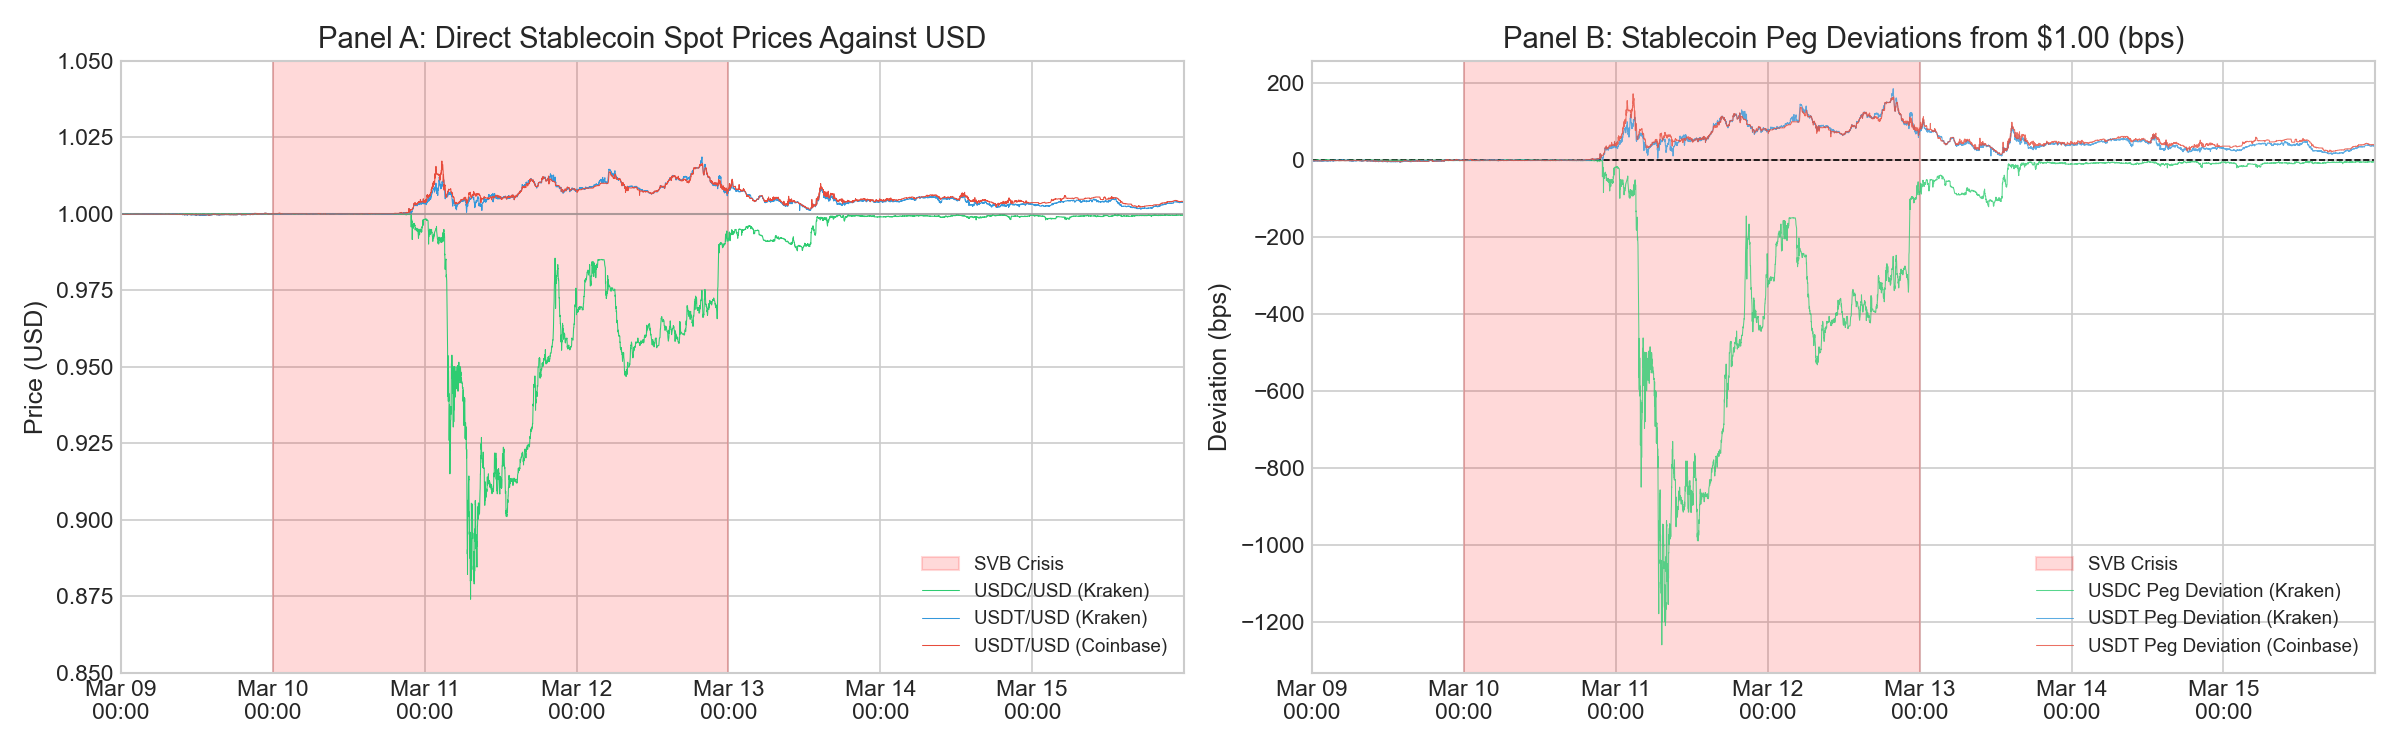
\includegraphics[width=1\linewidth]{figures/fig_stablecoin_peg.png}
    \caption{Stablecoin spot prices (A) and peg deviations in bps (B) during March 2023. USDC drops to \$0.874 while USDT trades at a premium. Shaded: SVB crisis window (March 10--13).}
    \label{fig:peg}
\end{figure}

\section{Data and Methodology}\label{sec:data}

\subsection{Data sources and preprocessing}
We collect 1-minute OHLCV candles for BTC quoted in USD, USDT, and USDC from Binance (BTC/USDT, BTC/USDC; dominant USDT volume), Coinbase (BTC/USD, BTC/USDT, USDT/USD; primary U.S.\ fiat gateway), and Kraken (BTC/USD, BTC/USDT, BTC/USDC, USDT/USD, USDC/USD; broadest stablecoin-to-fiat coverage). Stablecoin-to-USD conversion uses venue-specific legs. All series are aligned to a 1-minute UTC grid (Table~\ref{tab:data_coverage}). Coverage exceeds 97\% for most series, though pre-SVB Kraken BTC/USDC falls to 89.6\% with 42\% forward-fill share. Short gaps ($\le5$ min) are forward-filled; larger gaps remain NaN. Core directional signs are stable under strict no-FF filtering (crisis USDC $D_t>0$, USDT premium $>0$), though some magnitudes shift on thinner samples. We interpret high-frequency levels as directional unless no-FF retention is adequate.

\begin{table}[H]
\caption{Core series data coverage and forward-fill exposure. Coverage is the share of non-missing 1-minute observations on the unified UTC grid; forward-fill share is the percent of minutes filled by carry-forward (up to 5 minutes).}
\label{tab:data_coverage}
\footnotesize
\resizebox{\textwidth}{!}{%
\begin{tabular}{lrrrrr}
\toprule
Pair & Coverage Overall (\%) & Coverage Pre-SVB (\%) & Coverage Crisis (\%) & Coverage Post-SVB (\%) & Forward-Fill Share Overall (\%) \\
\midrule
Kraken BTC/USD & 99.98 & 100.00 & 100.00 & 99.95 & 0.18 \\
Kraken BTC/USDT & 98.44 & 97.36 & 99.81 & 99.06 & 30.84 \\
Kraken BTC/USDC & 94.05 & 89.62 & 99.79 & 96.57 & 42.07 \\
Kraken USDC/USD & 97.80 & 96.03 & 99.35 & 99.06 & 28.57 \\
Kraken USDT/USD & 99.98 & 100.00 & 100.00 & 99.95 & 0.91 \\
Coinbase BTC/USD & 99.10 & 97.90 & 100.00 & 100.00 & 0.06 \\
Coinbase BTC/USDT & 98.93 & 97.53 & 99.95 & 99.98 & 17.98 \\
Coinbase USDT/USD & 99.02 & 97.72 & 100.00 & 100.00 & 0.06 \\
Binance BTC/USDT & 100.00 & 100.00 & 100.00 & 100.00 & 0.00 \\
Binance BTC/USDC & 100.00 & 100.00 & 100.00 & 100.00 & 0.00 \\
\bottomrule
\end{tabular}%
}
\end{table}


We proxy transaction frictions using the intra-candle range:
\begin{equation}
    \text{Intra-minute Range (bps)} = \left( \frac{\text{High}_t - \text{Low}_t}{\text{Close}_t} \right)\times 10000.
\end{equation}
This is a coarse range proxy that mechanically loads on volatility and microstructure noise; we interpret it cautiously as a friction indicator, not a quoted bid--ask spread.

\subsection{Core quantitative objects}

For stablecoin $Q\in\{\text{USDC}, \text{USDT}\}$, we track two objects. The \emph{unadjusted dispersion}:
\begin{equation}
    D_{Q,t}=\left(\ln(P_{\text{BTC}/Q,t})-\ln(P_{\text{BTC/USD},t})\right)\times 10000,
\end{equation}
and the \emph{adjusted parity residual}:
\begin{equation}
    B_{Q,t}
    = \left(\ln(P_{\text{BTC}/Q,t}\times P_{Q/\text{USD},t})-\ln(P_{\text{BTC/USD},t})\right)\times 10000.
\end{equation}
These satisfy $B_{Q,t}=D_{Q,t}+10000\cdot\ln(P_{Q/\text{USD},t})$: large de-pegs mechanically drive $D_t$ while $B_t$ captures the residual after marking to USD. Both are computed intra-exchange; cross-venue deviations are studied separately. Basis and dispersion are in log-bps; peg deviations, ranges, and volatility summaries are in arithmetic bps.

\subsection{Mean-reversion dynamics}
We model $B_t$ as an OU process $dX_t = \theta(\mu - X_t)dt + \sigma dW_t$ and estimate the discrete AR(1) form $X_t = c + \rho X_{t-1} + \varepsilon_t$. Stationarity is checked with ADF tests (with large $N$, rejection is expected and serves as a baseline screen). The half-life uses the exact mapping:
\begin{equation}
    \tau_{1/2} = \frac{\ln(2)\,\Delta t}{-\ln(\rho)}, \quad 0<\rho<1.
\end{equation}
If $\rho \le 0$ or $\rho \ge 1$, half-life is undefined (NaN). The OU framework assumes Gaussian innovations; crisis-period $B_t$ exhibits substantial excess kurtosis (Section~\ref{sec:liq_vol}), so we use the AR(1) model solely for its half-life mapping, not as a full distributional model. We report robustness at 5-minute sampling and with forward-filled minutes removed.

\subsection{Price discovery framework}
For the two primary Kraken channels (BTC/USD vs.\ BTC/USDC and BTC/USD vs.\ BTC/USDT), we use synchronized 1-minute log-price levels, dropping forward-filled minutes. We test for cointegration with Johansen trace tests (constant restricted to the cointegration relation; lag order via BIC on the levels VAR) \cite{johansen1988,englegranger1987}. When rank $=1$, we estimate:
\begin{equation}
    \Delta \mathbf{p}_t = \alpha \beta^\top \mathbf{p}_{t-1} + \sum_{i=1}^{k_{\Delta}} \Gamma_i \Delta \mathbf{p}_{t-i} + \mathbf{u}_t.
\end{equation}
The market with smaller $|\alpha|$ adjusts less and is interpreted as the relative leader. We retain BH/FDR-corrected Granger tests on returns as secondary evidence only \cite{granger1969}; with 1-minute bars, asynchrony and large $N$ can overstate economic lead--lag strength.

\section{Empirical Results}\label{sec:results}

\subsection{Dispersion, adjusted residual, and mean reversion}

Before SVB, both $D_t$ and $B_t$ hover near zero. During the crisis (March 10--13 UTC), USDC dispersion jumps to $+320$ bps ($\sigma{=}323$) while the adjusted residual remains small ($+5.3$ bps, $\sigma{=}21$). USDT moves oppositely: $D_t{=}{-}57$ bps, $B_t{=}{+}0.7$ bps (Table~\ref{tab:dispersion_vs_adjusted}). Figure~\ref{fig:decomp} visualizes this: $D_t$ (orange) captures the peg shift while $B_t$ (blue) remains tightly mean-reverting.

\begin{figure}[t]
    \centering
    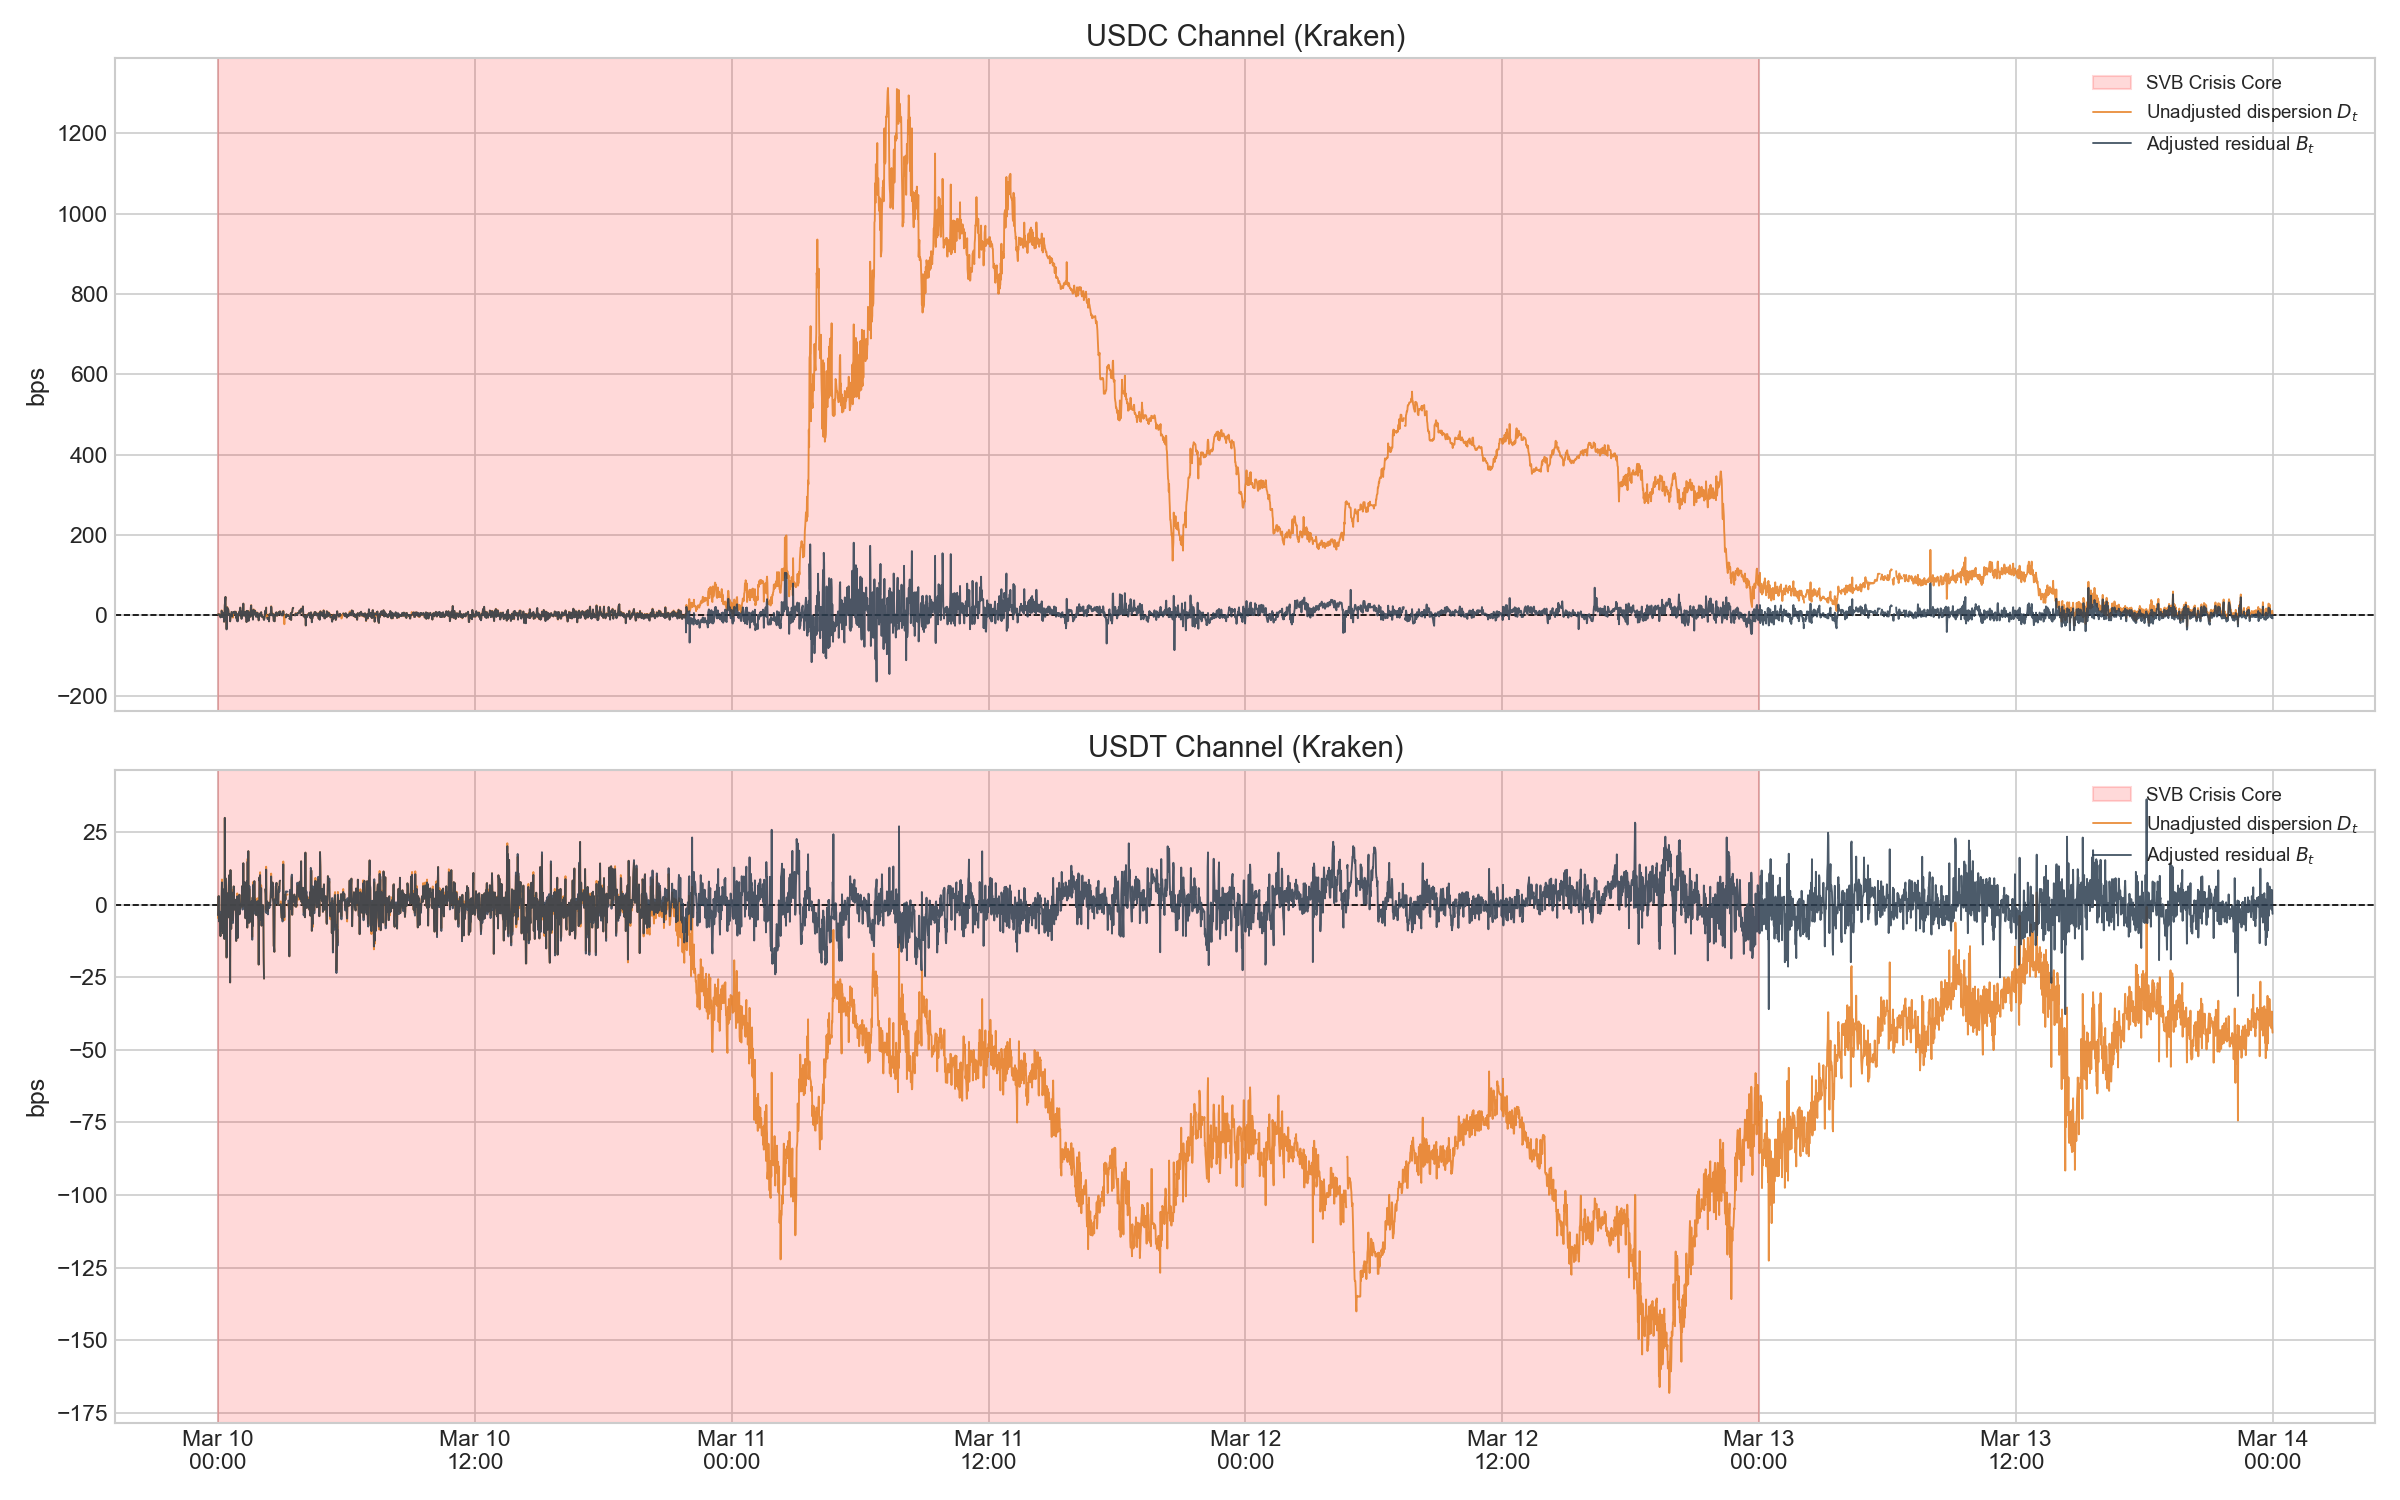
\includegraphics[width=0.92\linewidth]{figures/fig_dispersion_vs_adjusted_kraken.png}
    \caption{$D_t$ (orange) vs.\ $B_t$ (blue) on Kraken during crisis. Top: USDC---$D_t$ exceeds $+1{,}200$ bps while $B_t$ stays within $\pm150$ bps. Bottom: USDT---$D_t$ reflects the premium while $B_t\approx0$. The gap is attributable to the stablecoin peg deviation.}
    \label{fig:decomp}
\end{figure}

Two dynamics drive this pattern. USDC trades as low as \$0.874 on Kraken on March 11 (${\approx}{-}1{,}260$ bps), mechanically pulling $D_t$ upward; simultaneously, USDT trades at a premium averaging $+58.1$ bps on Kraken and $+59.7$ on Coinbase. Figure~\ref{fig:substitution} visualizes this stablecoin substitution: crisis observations (red) migrate to the lower-right quadrant ($D_{\text{USDC}}>0$, $D_{\text{USDT}}<0$), and the unadjusted cross-stablecoin correlation flips from $+0.44$ to $-0.42$---consistent with traders rotating out of USDC into USDT under stress.

\begin{figure}[t]
    \centering
    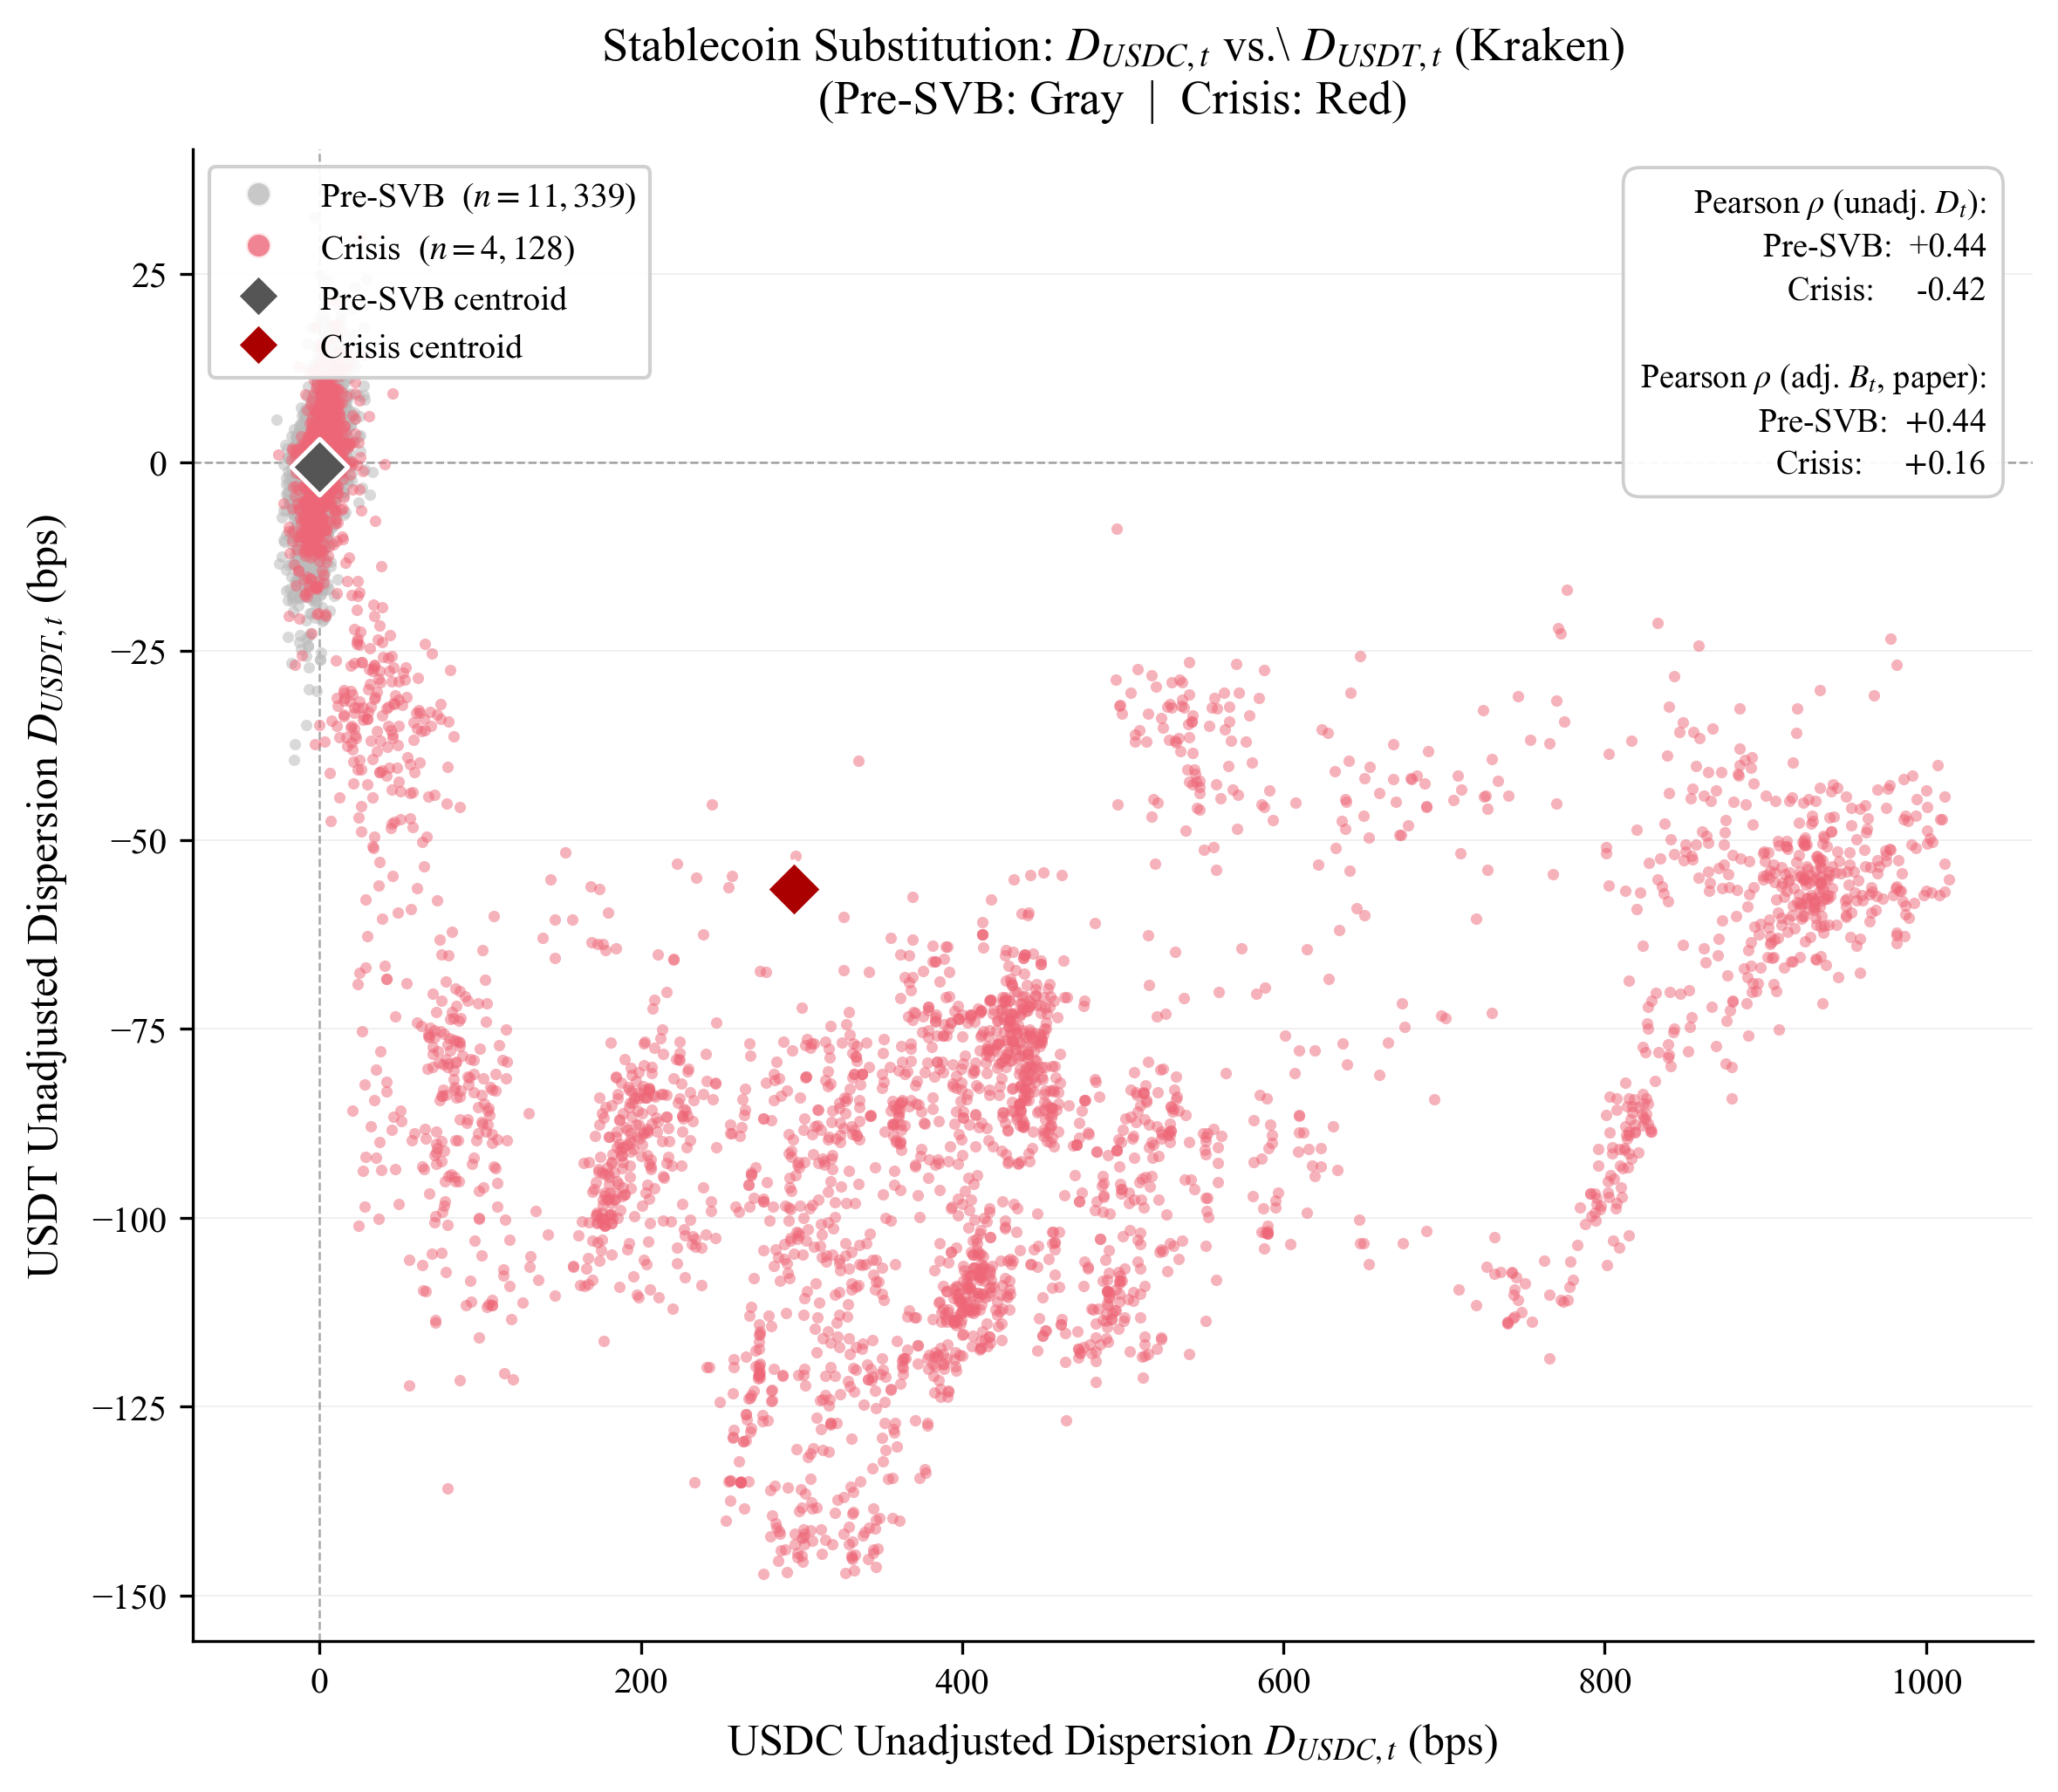
\includegraphics[width=0.75\linewidth]{figures/fig_stablecoin_substitution_scatter.png}
    \caption{Stablecoin substitution: $D_{\text{USDC},t}$ vs.\ $D_{\text{USDT},t}$ on Kraken. Pre-SVB (gray) clusters near the origin; crisis (red) migrates to the lower-right quadrant. Unadjusted correlation flips from $+0.44$ to $-0.42$; adjusted $B_t$ correlation drops from $0.44$ to $0.16$.}
    \label{fig:substitution}
\end{figure}

\begin{table}
\caption{Regime Statistics for Unadjusted Dispersion ($D_t$) and Adjusted Residual ($B_t$), Kraken}
\label{tab:dispersion_vs_adjusted}
\begin{tabular}{llrrrr}
\toprule
Regime & Series & Mean (bps) & Std (bps) & Mean Abs (bps) & N \\
\midrule
Pre-SVB & USDC Kraken $D_t$ (Unadjusted) & 0.12 & 4.95 & 3.49 & 11615 \\
Pre-SVB & USDC Kraken $B_t$ (Adjusted) & -0.32 & 5.00 & 3.53 & 11197 \\
Pre-SVB & USDT Kraken $D_t$ (Unadjusted) & -0.54 & 4.49 & 3.17 & 12618 \\
Pre-SVB & USDT Kraken $B_t$ (Adjusted) & -0.60 & 4.33 & 3.02 & 12618 \\
Crisis & USDC Kraken $D_t$ (Unadjusted) & 319.97 & 322.87 & 321.17 & 4311 \\
Crisis & USDC Kraken $B_t$ (Adjusted) & 5.27 & 21.21 & 13.37 & 4283 \\
Crisis & USDT Kraken $D_t$ (Unadjusted) & -57.18 & 45.10 & 58.57 & 4312 \\
Crisis & USDT Kraken $B_t$ (Adjusted) & 0.68 & 6.57 & 4.94 & 4312 \\
Post-SVB & USDC Kraken $D_t$ (Unadjusted) & 11.22 & 21.95 & 14.27 & 12514 \\
Post-SVB & USDC Kraken $B_t$ (Adjusted) & 0.45 & 9.06 & 6.68 & 12419 \\
Post-SVB & USDT Kraken $D_t$ (Unadjusted) & -30.26 & 13.29 & 30.28 & 12837 \\
Post-SVB & USDT Kraken $B_t$ (Adjusted) & -1.23 & 6.47 & 4.92 & 12837 \\
\bottomrule
\end{tabular}
\end{table}


HAC/Newey--West intervals (60-lag cap) confirm directional robustness \cite{neweywest1987}: USDC crisis $D_t$ 95\% CI $[245.7,\,394.3]$ bps; crisis $B_t$ CI $[3.6,\,7.0]$ bps; USDT premiums positive on both Kraken ($[47.4,\,68.8]$) and Coinbase ($[49.1,\,70.3]$). Coinbase--Kraken BTC/USD remains significantly positive ($[1.7,\,2.6]$ bps).

ADF rejects a unit root for all $B_t$ channels ($p<0.001$). Kraken USDC half-life: $0.98$ min pre-SVB, $0.61$ min crisis, $0.79$ min post-SVB. Figure~\ref{fig:halflife_robust} shows robustness across 1m/5m sampling and all/no-FF filters: USDC crisis half-life ranges from $0.54$ to $1.10$ min; USDT crisis half-life is longer ($0.92$--$3.06$ min). Fast USDC mean reversion is robust across all specifications.

\begin{figure}[t]
    \centering
    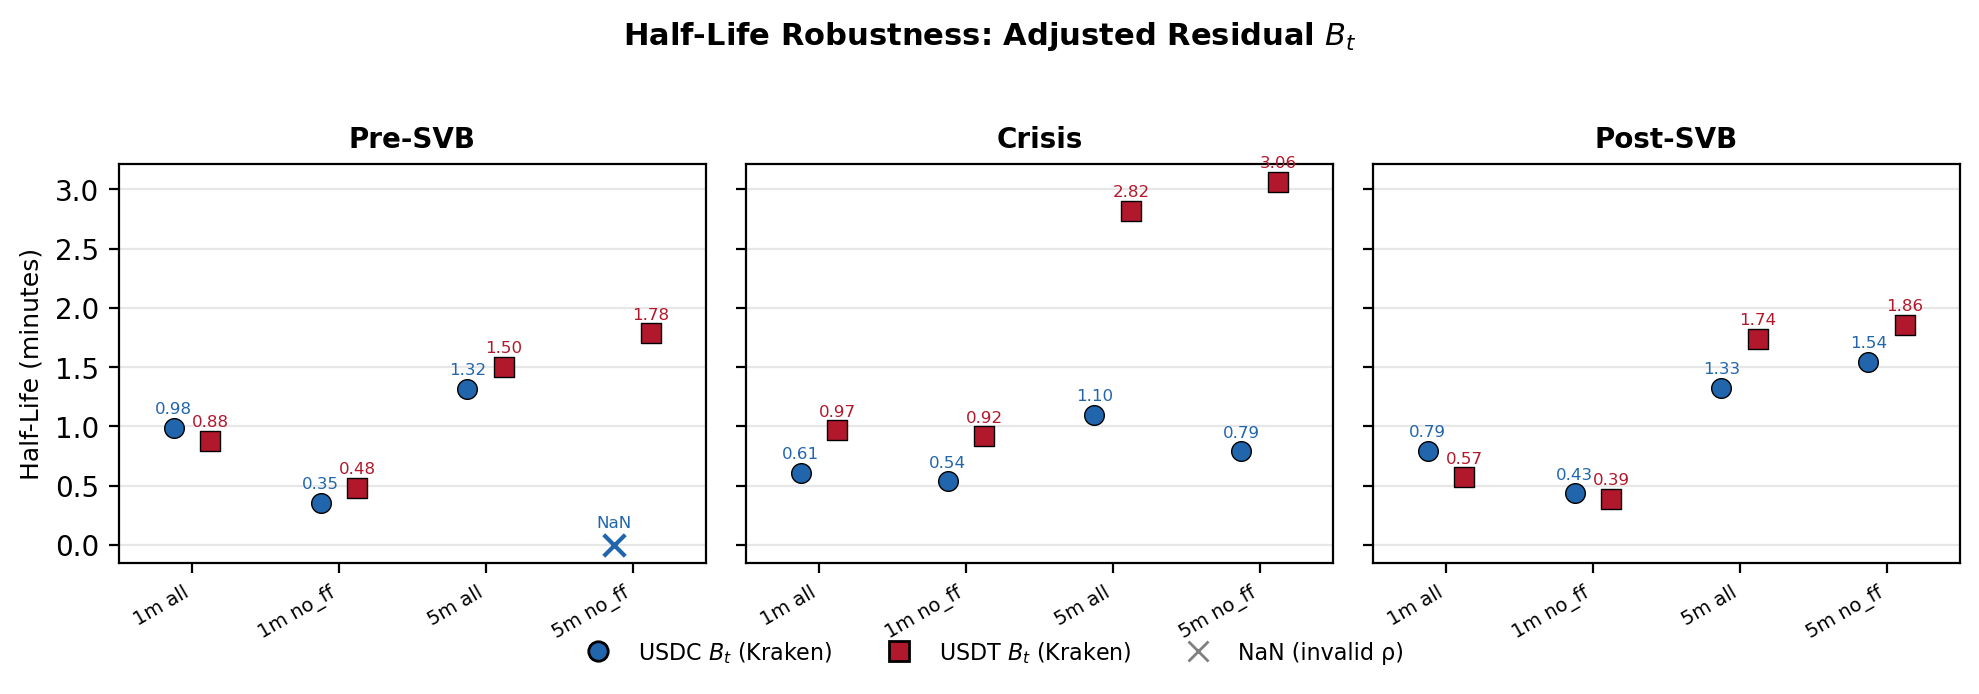
\includegraphics[width=0.92\linewidth]{figures/fig_half_life_robustness.png}
    \caption{Half-life robustness for adjusted residual $B_t$: USDC (blue circles) vs.\ USDT (red squares) across four specifications (1m/5m $\times$ all/no-FF) and three regimes. USDC crisis half-life is consistently below 1.1 min; USDT crisis half-life reaches 3.1 min at 5m no-FF.}
    \label{fig:halflife_robust}
\end{figure}

The OU estimation reveals a \textbf{two-layer dynamic} (Figure~\ref{fig:twolayer}): $B_t$ mean-reverts in ${\approx}0.6$ min during crisis ($\hat\rho{=}0.320$), while the USDC peg deviation persists with half-life ${\approx}572$ min ($\hat\rho{=}0.999$, ADF $p{=}0.44$); USDT peg deviations similarly persist ($496$--$542$ min). This ${\sim}940\times$ gap shows cross-market correction is fast even in crisis, but the peg itself---driven by reserve-access risk---is where dislocation persists.

\begin{figure}[t]
    \centering
    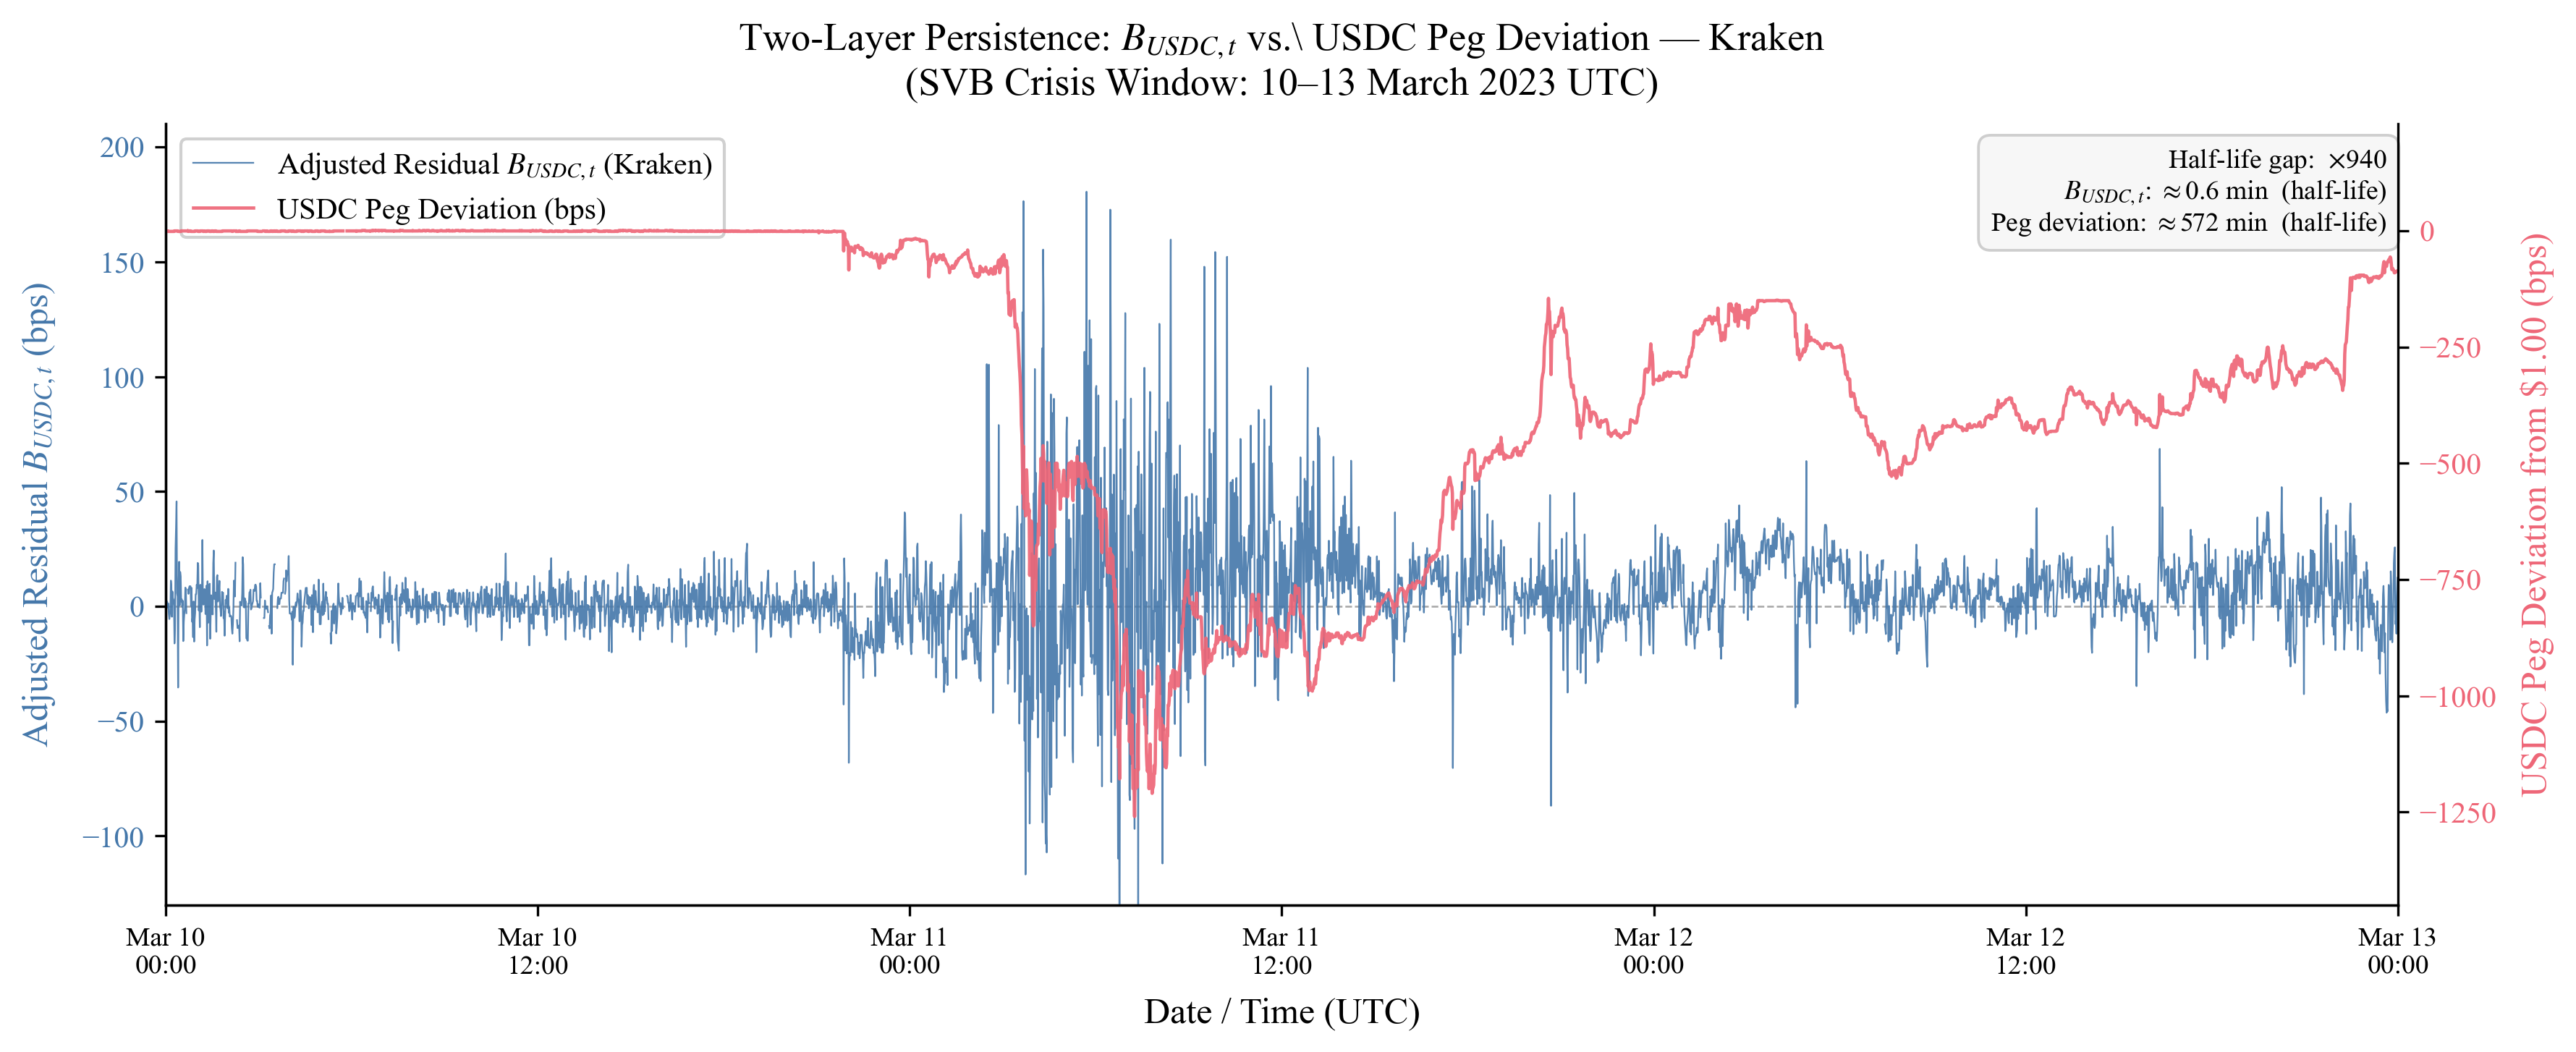
\includegraphics[width=0.92\linewidth]{figures/fig_two_layer_persistence.png}
    \caption{Two-layer persistence (March 10--13). $B_{\text{USDC},t}$ (blue, left) mean-reverts in ${\approx}0.6$ min; USDC peg deviation (red, right) persists for hours (${\approx}572$ min). The ${\sim}940\times$ gap localizes dislocation to the peg layer.}
    \label{fig:twolayer}
\end{figure}

Figure~\ref{fig:crisiszoom} provides a granular minute-by-minute view of all channels during the peak crisis window. Panel~A reveals that the USDC adjusted residual (green) exhibits extreme volatility---spikes exceeding $+150$ bps---while the USDT channels on both Kraken and Coinbase remain tightly bounded near zero throughout. This asymmetry reinforces the finding that the crisis is USDC-specific rather than a broad market dislocation. Panel~B shows that cross-exchange differentials widen simultaneously, with the Coinbase--Kraken BTC/USD basis rising to $+60$ bps, suggesting stress propagation across venues---a pattern we examine in the next subsection.

\begin{figure}[t]
    \centering
    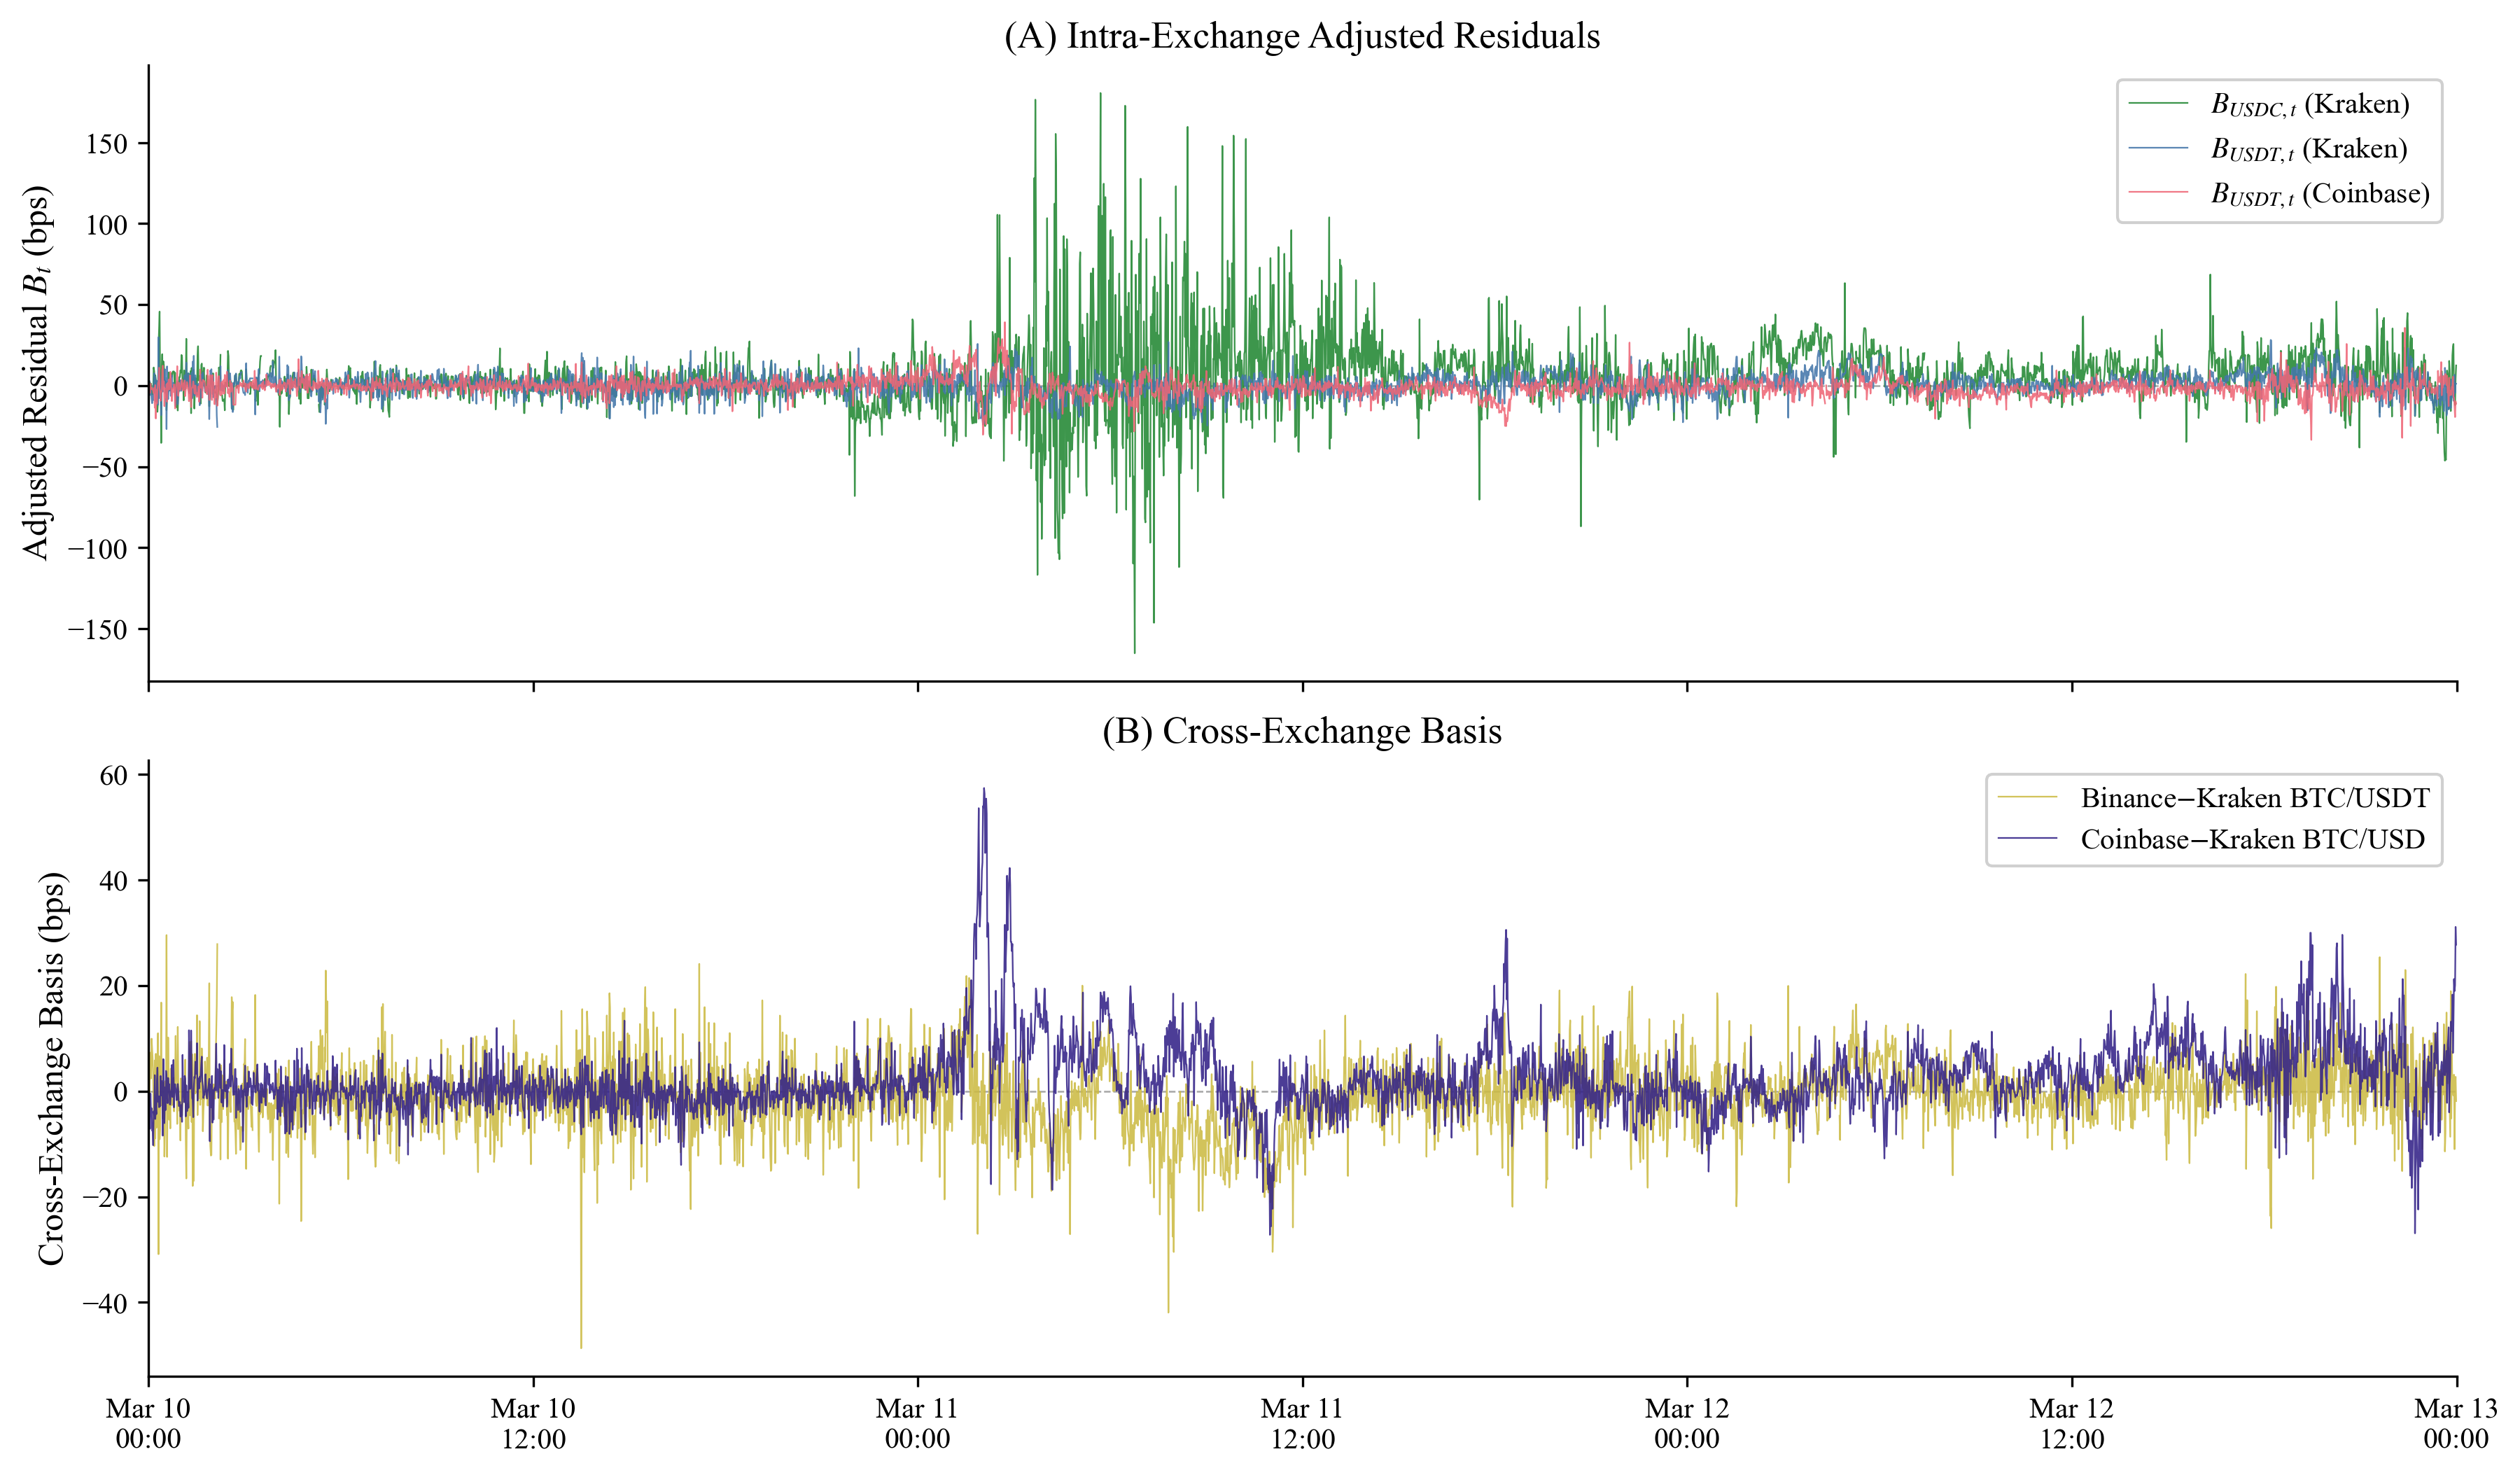
\includegraphics[width=0.92\linewidth]{figures/fig_svb_crisis_zoom.png}
    \caption{Minute-level crisis zoom (March 10--13 UTC). (A)~Intra-exchange adjusted residuals: $B_{\text{USDC},t}$ (Kraken, green) spikes past $\pm150$ bps while USDT channels stay within $\pm30$ bps. (B)~Cross-exchange basis: both Binance--Kraken BTC/USDT and Coinbase--Kraken BTC/USD widen, indicating stress propagation across venues.}
    \label{fig:crisiszoom}
\end{figure}

\subsection{Cross-exchange price dispersion}
Having established that intra-exchange fragmentation is dominated by USDC peg risk, a natural question is whether this dislocation propagates \emph{across} exchanges. We examine this by computing log-price differentials for BTC/USDT (Binance vs.\ Kraken; Coinbase vs.\ Kraken) and BTC/USD (Coinbase vs.\ Kraken). Caveat: USDT cross-exchange dispersion is in the USDT numeraire; a USD-based arbitrage requires an additional USDT/USD leg. Binance--Kraken BTC/USDT is near zero full-sample ($+0.007$ bps), consistent with tight integration. Coinbase--Kraken BTC/USD shows a persistent $+2.18$ bps premium, consistent with a structural U.S.\ fiat gateway effect.

During the crisis, cross-exchange differentials widen alongside intra-exchange deviations (Figure~\ref{fig:xbasis}, Table~\ref{tab:arb}), consistent with broad stress rather than a single-venue disruption. The Coinbase--Kraken fiat premium did not fully normalize post-crisis, suggesting it partly reflects structural microstructure differences that stress amplified.

\begin{figure}[t]
    \centering
    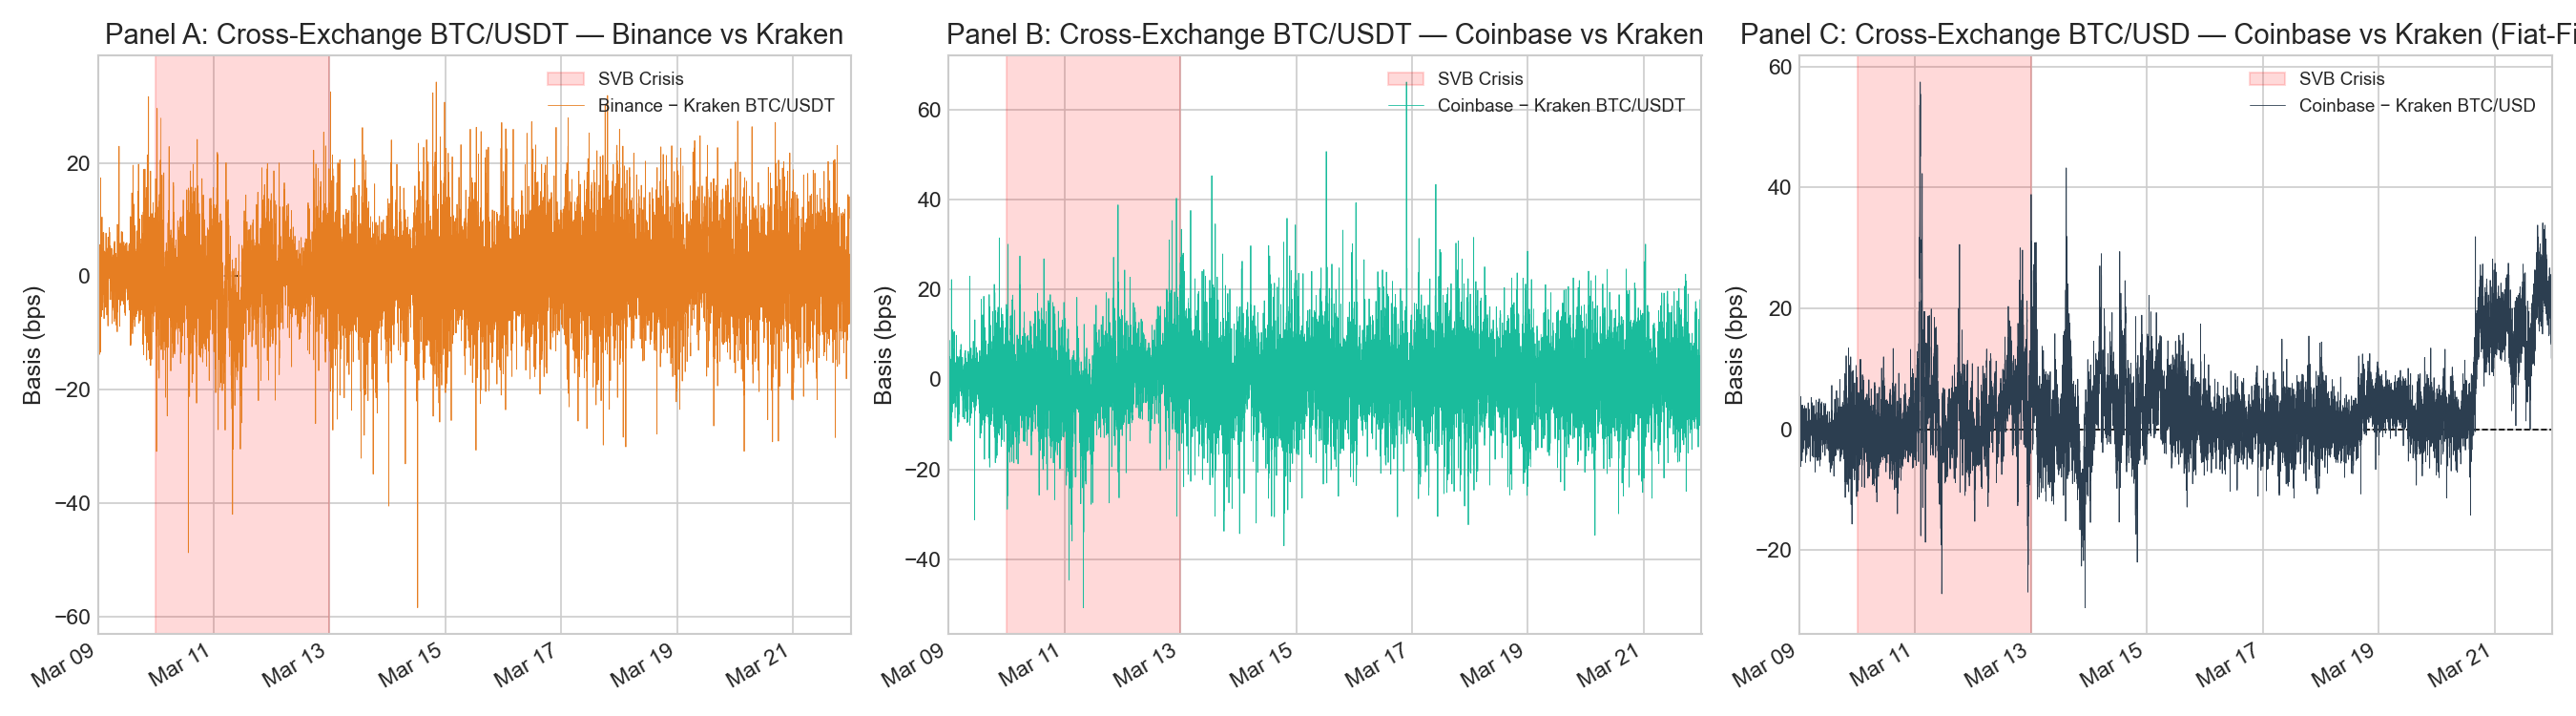
\includegraphics[width=0.92\linewidth]{figures/fig_cross_exchange_basis.png}
    \caption{Cross-exchange basis (bps): BTC/USDT Binance--Kraken (A), Coinbase--Kraken (B), and BTC/USD Coinbase--Kraken (C). The fiat channel shows a persistent positive basis that remains elevated post-crisis, suggesting structural microstructure differences.}
    \label{fig:xbasis}
\end{figure}

\subsection{Market microstructure dynamics}\label{sec:liq_vol}
The cross-exchange widening documented above raises the question of whether liquidity conditions differ materially across channels. We quantify liquidity with the Roll (1984) effective spread \cite{roll1984} and Amihud (2002) ILLIQ ratio \cite{amihud2002}. Table~\ref{tab:liquidity_spread} and Figure~\ref{fig:liq} report regime means. Kraken BTC/USDC Roll spread jumps $23\times$ ($1.10$ to $25.64$ bps), while BTC/USDT holds near $3$ bps. Amihud confirms Coinbase BTC/USD is deepest and Kraken BTC/USDC least liquid. The two measures diverge in crisis: Roll widens while Amihud declines as volume surges.

\begin{figure}[t]
    \centering
    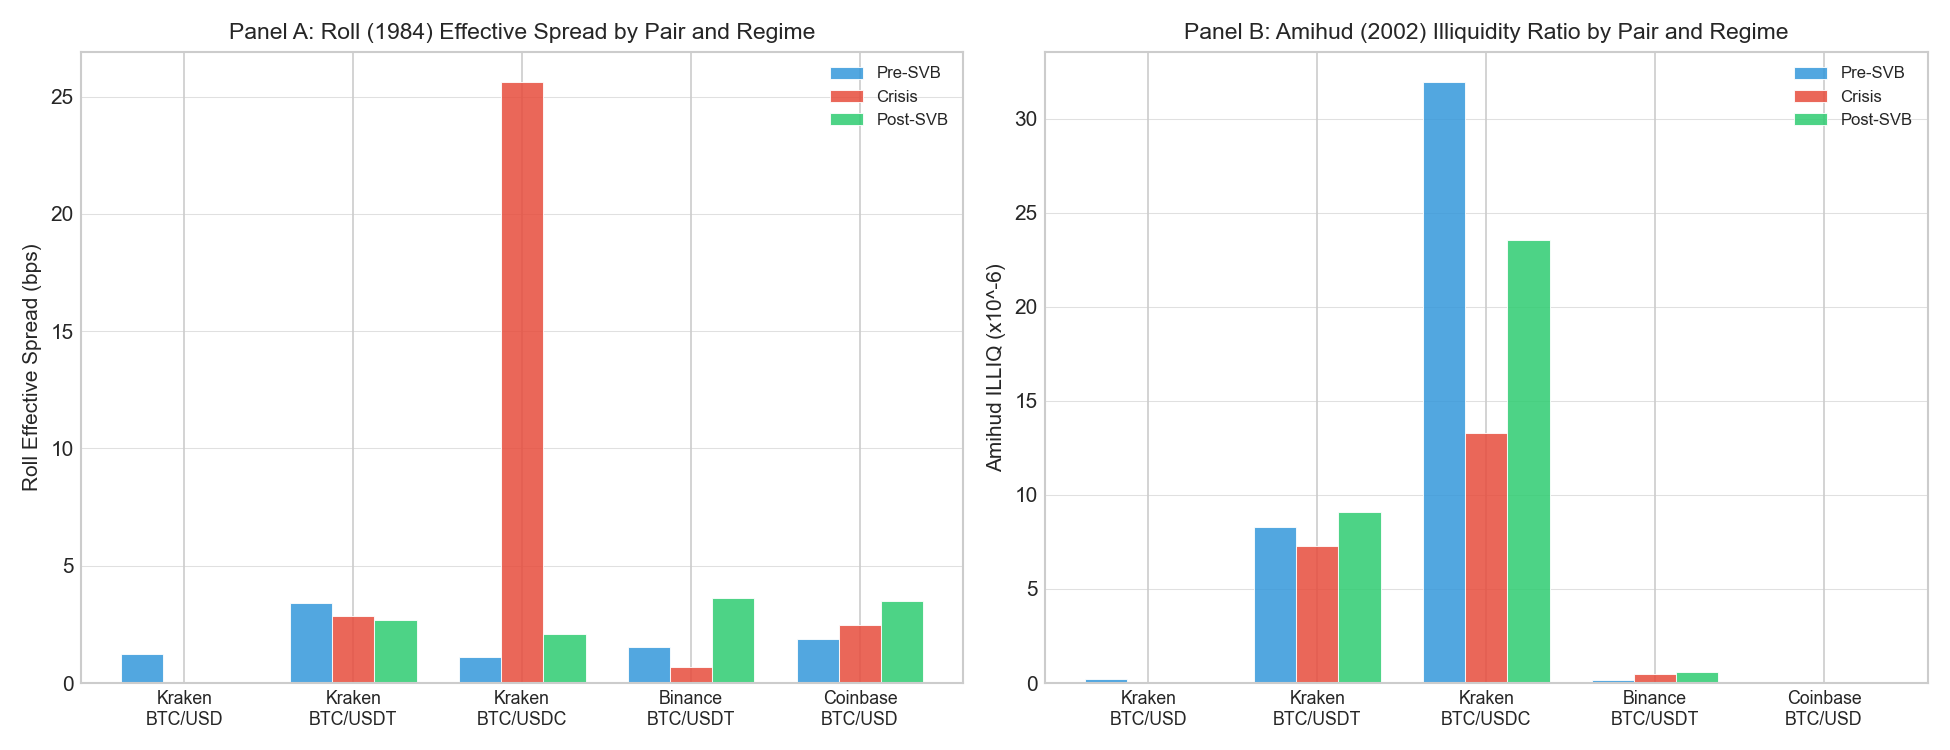
\includegraphics[width=0.92\linewidth]{figures/fig_liquidity_roll_amihud.png}
    \caption{Roll (1984) effective spread (A) and Amihud (2002) ILLIQ ratio (B) by pair and regime. Kraken BTC/USDC shows a $23\times$ Roll spread blowout in crisis. Roll is undefined when serial covariance is non-negative; regime means for thin pairs rest on few valid days and are indicative.}
    \label{fig:liq}
\end{figure}

\begin{table}[H]
\caption{Roll (1984) effective spread (bps) and Amihud (2002) illiquidity ratio ($\times10^{-6}$) by pair and regime. Roll spread estimated from daily serial covariance of 1-minute log returns; NaN days (non-negative covariance) excluded from means. $N$ is the number of valid Roll days per regime; some regime means rest on few days and are indicative. ILLIQ$_t = |r_t|/\text{DollarVol}_t$, daily average.}
\label{tab:liquidity_spread}
\footnotesize
\resizebox{\textwidth}{!}{%
\begin{tabular}{lrrrrrrrrr}
\toprule
Pair & Roll\textsubscript{Pre} & Roll\textsubscript{Crisis} & Roll\textsubscript{Post} & $N$\textsubscript{Pre} & $N$\textsubscript{Crisis} & $N$\textsubscript{Post} & ILLIQ\textsubscript{Pre} & ILLIQ\textsubscript{Crisis} & ILLIQ\textsubscript{Post} \\
\midrule
Kraken BTC/USD & 1.260 & --- & --- & 4 & 0 & 0 & 0.232 & 0.050 & 0.068 \\
Kraken BTC/USDT & 3.390 & 2.850 & 2.670 & 1 & 1 & 1 & 8.299 & 7.266 & 9.074 \\
Kraken BTC/USDC & 1.100 & 25.640 & 2.070 & 2 & 2 & 2 & 31.970 & 13.282 & 23.530 \\
Binance BTC/USDT & 1.560 & 0.670 & 3.630 & 6 & 1 & 5 & 0.163 & 0.461 & 0.591 \\
Coinbase BTC/USD & 1.880 & 2.490 & 3.490 & 5 & 1 & 1 & 0.005 & 0.003 & 0.003 \\
\bottomrule
\end{tabular}%
}
\end{table}


Daily dollar-volume depth proxies (Table~\ref{tab:depth_proxy}) sharpen this picture: Coinbase BTC/USD is the deepest channel (\$239M pre-SVB, rising to \$664M post-SVB), while Kraken BTC/USDC is $26\times$ thinner in crisis (\$15.7M vs.\ \$407M). The depth gap constrains the scale at which arbitrageurs can trade the USDC dislocation, consistent with the limited post-friction profitability documented in Section~\ref{sec:arb}.

\begin{table}[H]
\caption{Daily traded dollar volume depth proxy by pair and regime (median, USD millions/day). Because historical L2 order-book snapshots are unavailable in the candle APIs used here, dollar volume and Amihud ILLIQ are used as complementary depth proxies.}
\label{tab:depth_proxy}
\footnotesize
\resizebox{\textwidth}{!}{%
\begin{tabular}{lrrr}
\toprule
Pair & Median DollarVol Pre-SVB ($MM/day$) & Median DollarVol Crisis ($MM/day$) & Median DollarVol Post-SVB ($MM/day$) \\
\midrule
Kraken BTC/USD & 59.50 & 160.36 & 203.77 \\
Kraken BTC/USDT & 5.55 & 13.84 & 17.37 \\
Kraken BTC/USDC & 2.56 & 15.65 & 5.52 \\
Binance BTC/USDT & 52.44 & 73.92 & 71.46 \\
Coinbase BTC/USD & 239.07 & 407.27 & 664.46 \\
\bottomrule
\end{tabular}%
}
\end{table}


HAC regressions (Newey--West, 60 lags) of $B_t$ on a crisis dummy, realized volatility, and range proxy (Table~\ref{tab:regression_hac}) show a significant USDC crisis coefficient ($+4.30$ bps, $p<0.001$) \cite{neweywest1987}. Explanatory power is modest ($R^2=0.041$), so we interpret these as partial associations.

\begin{table}[H]
\caption{HAC Regressions of Adjusted Residual $B_t$ on Crisis Dummy, Realized Volatility, and Range Proxy (Kraken, Newey--West 60 lags)}
\label{tab:regression_hac}
\footnotesize
\centering
\begin{tabular}{lcccc}
\toprule
 & \multicolumn{2}{c}{USDC Channel} & \multicolumn{2}{c}{USDT Channel} \\
\cmidrule(lr){2-3} \cmidrule(lr){4-5}
 & Coef. & $p$-value & Coef. & $p$-value \\
\midrule
Constant          & $-0.079$ & 0.833 & $-0.656$ & $<0.001$ \\
Crisis            & $+4.295$ & $<0.001$ & $+1.655$ & $<0.001$ \\
RealizedVol (60m) & $+0.004$ & 0.928 & $-0.029$ & 0.179 \\
Range Proxy       & $+0.048$ & 0.005 & $-0.013$ & 0.082 \\
\midrule
$R^2$             & \multicolumn{2}{c}{0.041} & \multicolumn{2}{c}{0.012} \\
$N$               & \multicolumn{2}{c}{26,489} & \multicolumn{2}{c}{26,489} \\
\bottomrule
\multicolumn{5}{l}{\footnotesize OLS with HAC standard errors (Newey--West, 60 lags). Dependent variable: $B_t$ (bps).}
\end{tabular}
\end{table}


Figure~\ref{fig:volshare} shows daily volume fragmentation: USDC share doubles during crisis (2.1\% to 4.3\%) as activity concentrates in Kraken BTC/USDC, while post-crisis USD dominance returns (86.9\%).

\begin{figure}[t]
    \centering
    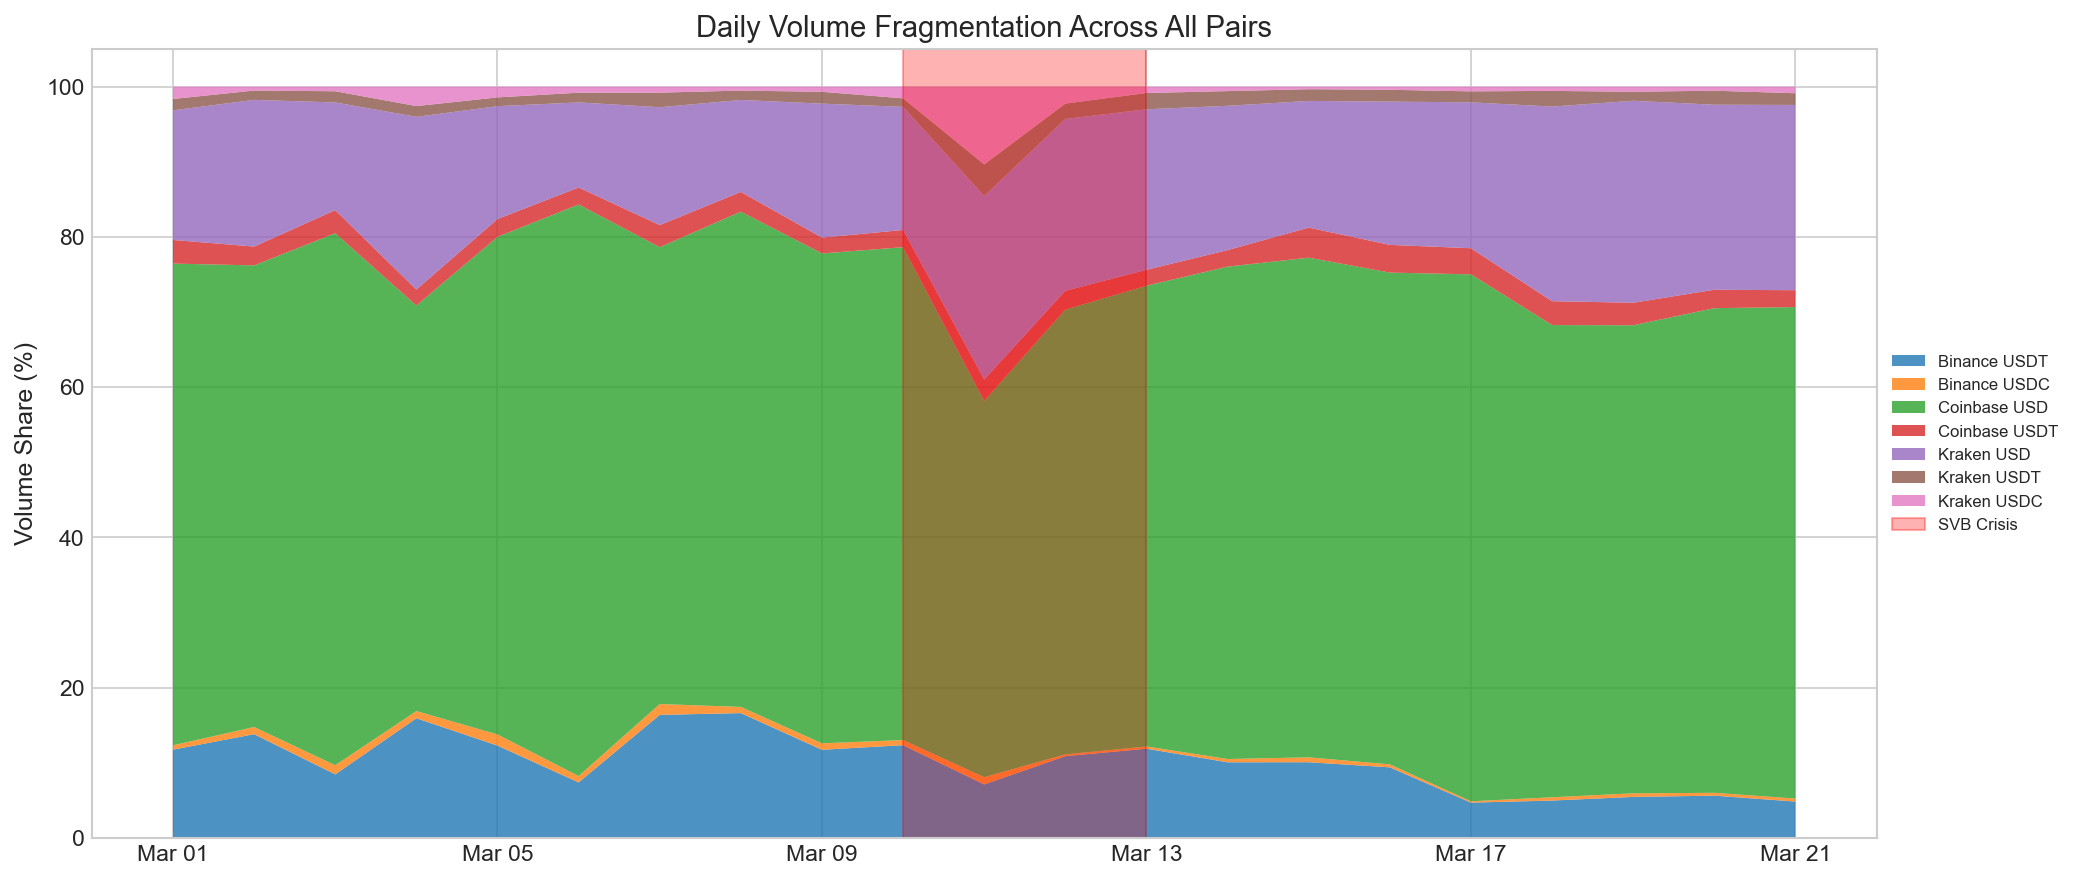
\includegraphics[width=0.92\linewidth]{figures/fig_volume_share.png}
    \caption{Daily volume fragmentation across all pairs. USDC share spikes during crisis as Kraken BTC/USDC activity surges; post-crisis, volume rotates back to USD dominance.}
    \label{fig:volshare}
\end{figure}

Realized volatility (Figure~\ref{fig:realvol}) reveals pronounced asymmetry: Kraken BTC/USDC peaks at ${\approx}650$ bps/hr on March 11, roughly $2.1\times$ the crisis-average for BTC/USD and BTC/USDT---consistent with compounding asset risk and numeraire risk.

\begin{figure}[t]
    \centering
    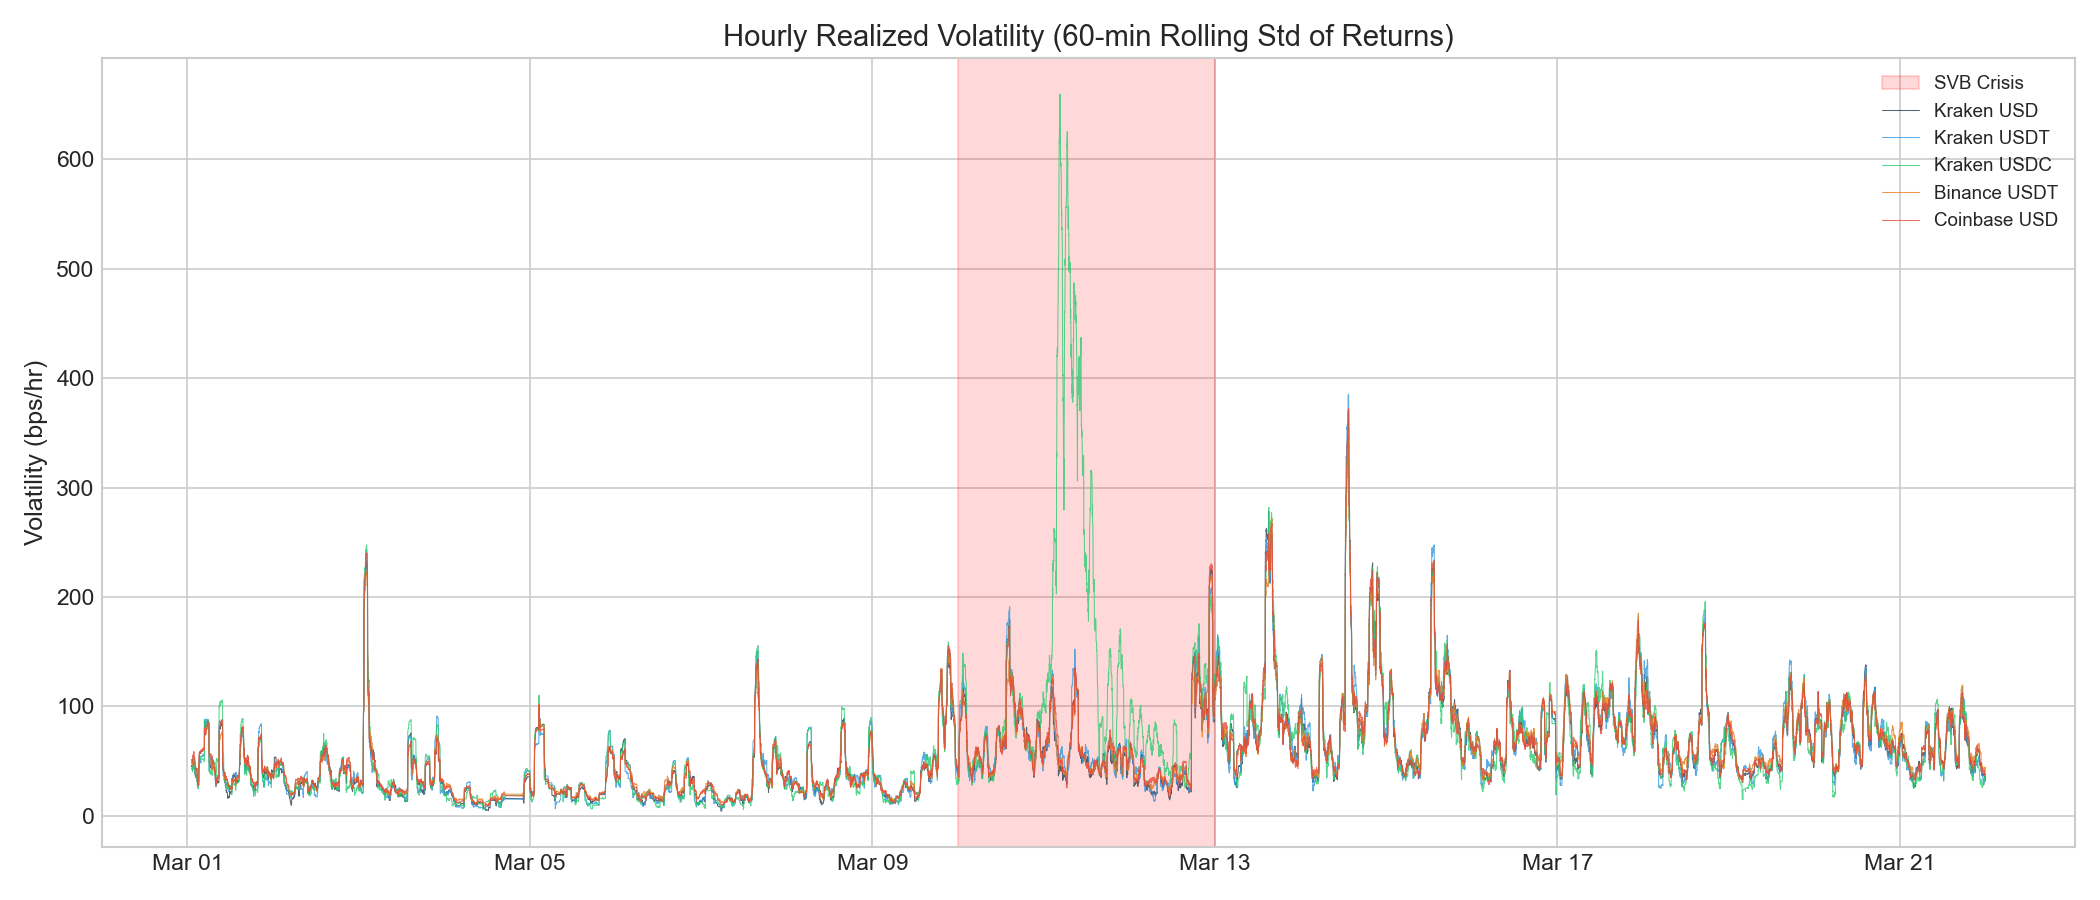
\includegraphics[width=0.92\linewidth]{figures/fig_realized_volatility.png}
    \caption{Hourly realized volatility (60-min rolling $\sigma$, $\times\sqrt{60}$) by pair. Kraken BTC/USDC (green) peaks at ${\approx}650$ bps/hr during crisis, roughly $2.1\times$ the USD and USDT channels, consistent with compounding asset and numeraire risk.}
    \label{fig:realvol}
\end{figure}

The distributional impact is stark (Figure~\ref{fig:tailblowout}): crisis USDC $B_t$ develops tails beyond $\pm100$ bps versus $\pm10$ bps pre-SVB. For risk management, stablecoin positions carry latent peg-break tail risk that calm-calibrated VaR models materially understate.

\begin{figure}[t]
    \centering
    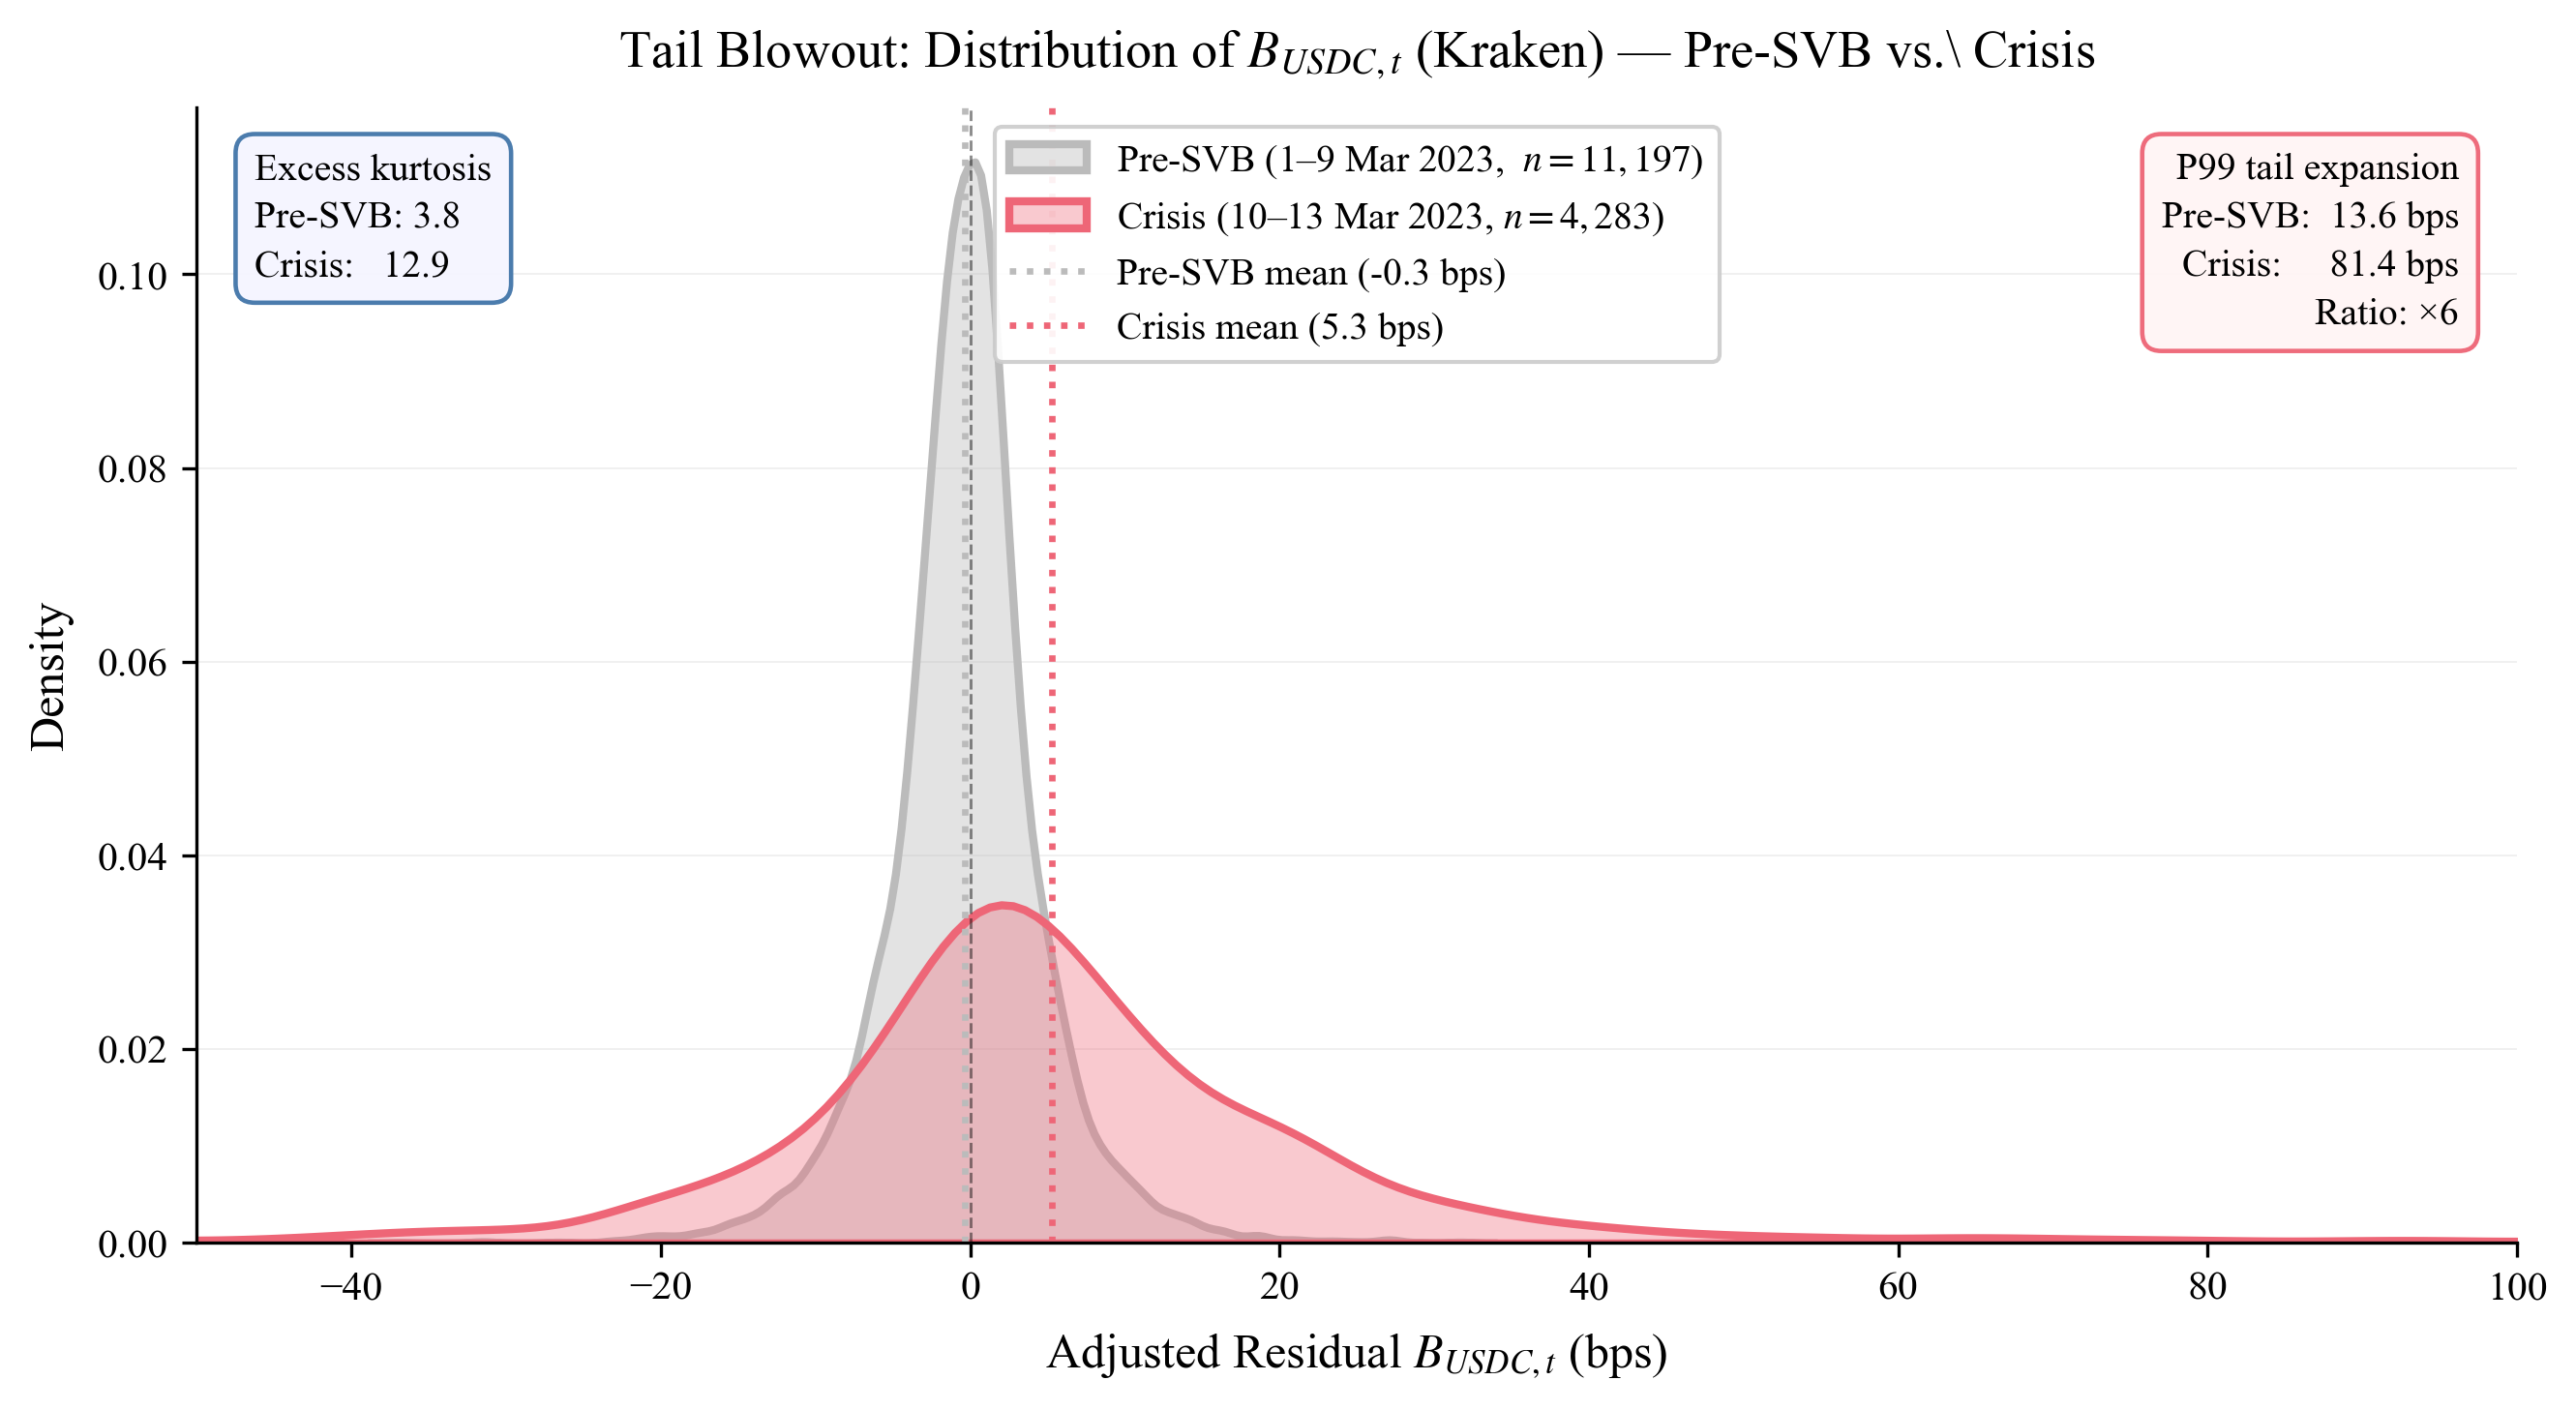
\includegraphics[width=0.85\linewidth]{figures/fig_tail_blowout_kde.png}
    \caption{Distribution of the USDC adjusted residual $B_{\text{USDC},t}$ on Kraken: pre-SVB (gray) versus crisis (red). The crisis distribution exhibits a rightward shift, excess kurtosis of 12.9 (vs.\ 3.8 pre-SVB), and a $6\times$ expansion in the 99th percentile (from 13.6 to 81.4 bps), confirming USDC-specific tail risk.}
    \label{fig:tailblowout}
\end{figure}

\paragraph{Distributional robustness.}
\begin{sloppypar}
Chow tests reject parameter stability at March~10 for $D_t$ ($F{=}2{,}089$), $B_t$ ($F{=}230$), and AR(1) dynamics ($F{=}71$; all $p{<}10^{-16}$), validating the regime split \cite{chow1960}. Table~\ref{tab:dist_robust}: USDC crisis $B_t$ has excess kurtosis 12.9 and skewness $+1.01$ (vs.\ pre-SVB 3.8/${\approx}$0); USDT crisis kurtosis is only 1.4---confirming USDC-specific tail risk. Jarque--Bera rejects normality throughout (USDC crisis JB${=}$30,498). Cross-stablecoin correlation drops from 0.44 to 0.16 in crisis, consistent with divergent dynamics rather than a common shock.
\end{sloppypar}

\begin{table}[H]
\caption{Higher-moment diagnostics for adjusted residual $B_t$ by regime. Excess kurtosis (Fisher) measures tail heaviness beyond Gaussian ($=0$). Min/Max are in basis points.}
\label{tab:dist_robust}
\footnotesize
\begin{tabular}{llrrrr}
\toprule
Channel & Regime & Skewness & Ex.~Kurt. & Min & Max \\
\midrule
USDC & Pre-SVB & 0.00 & 3.8 & -36.9 & 32.0 \\
USDC & Crisis & 1.01 & 12.9 & -165.2 & 180.6 \\
USDC & Post-SVB & 0.30 & 2.8 & -43.2 & 79.4 \\
USDT & Pre-SVB & -0.36 & 5.2 & -36.4 & 34.5 \\
USDT & Crisis & -0.11 & 1.4 & -26.8 & 29.9 \\
USDT & Post-SVB & -0.03 & 2.0 & -37.8 & 36.2 \\
\bottomrule
\end{tabular}
\end{table}


Figure~\ref{fig:corrheat} visualizes the decorrelation across all channels: pre-SVB cross-channel correlations ($B_{\text{USDC}}$--$B_{\text{USDT}}$: $0.44$) collapse in crisis ($0.16$) and partially recover post-SVB ($0.38$), while cross-exchange USDT channels remain tightly correlated throughout.

\begin{figure}[t]
    \centering
    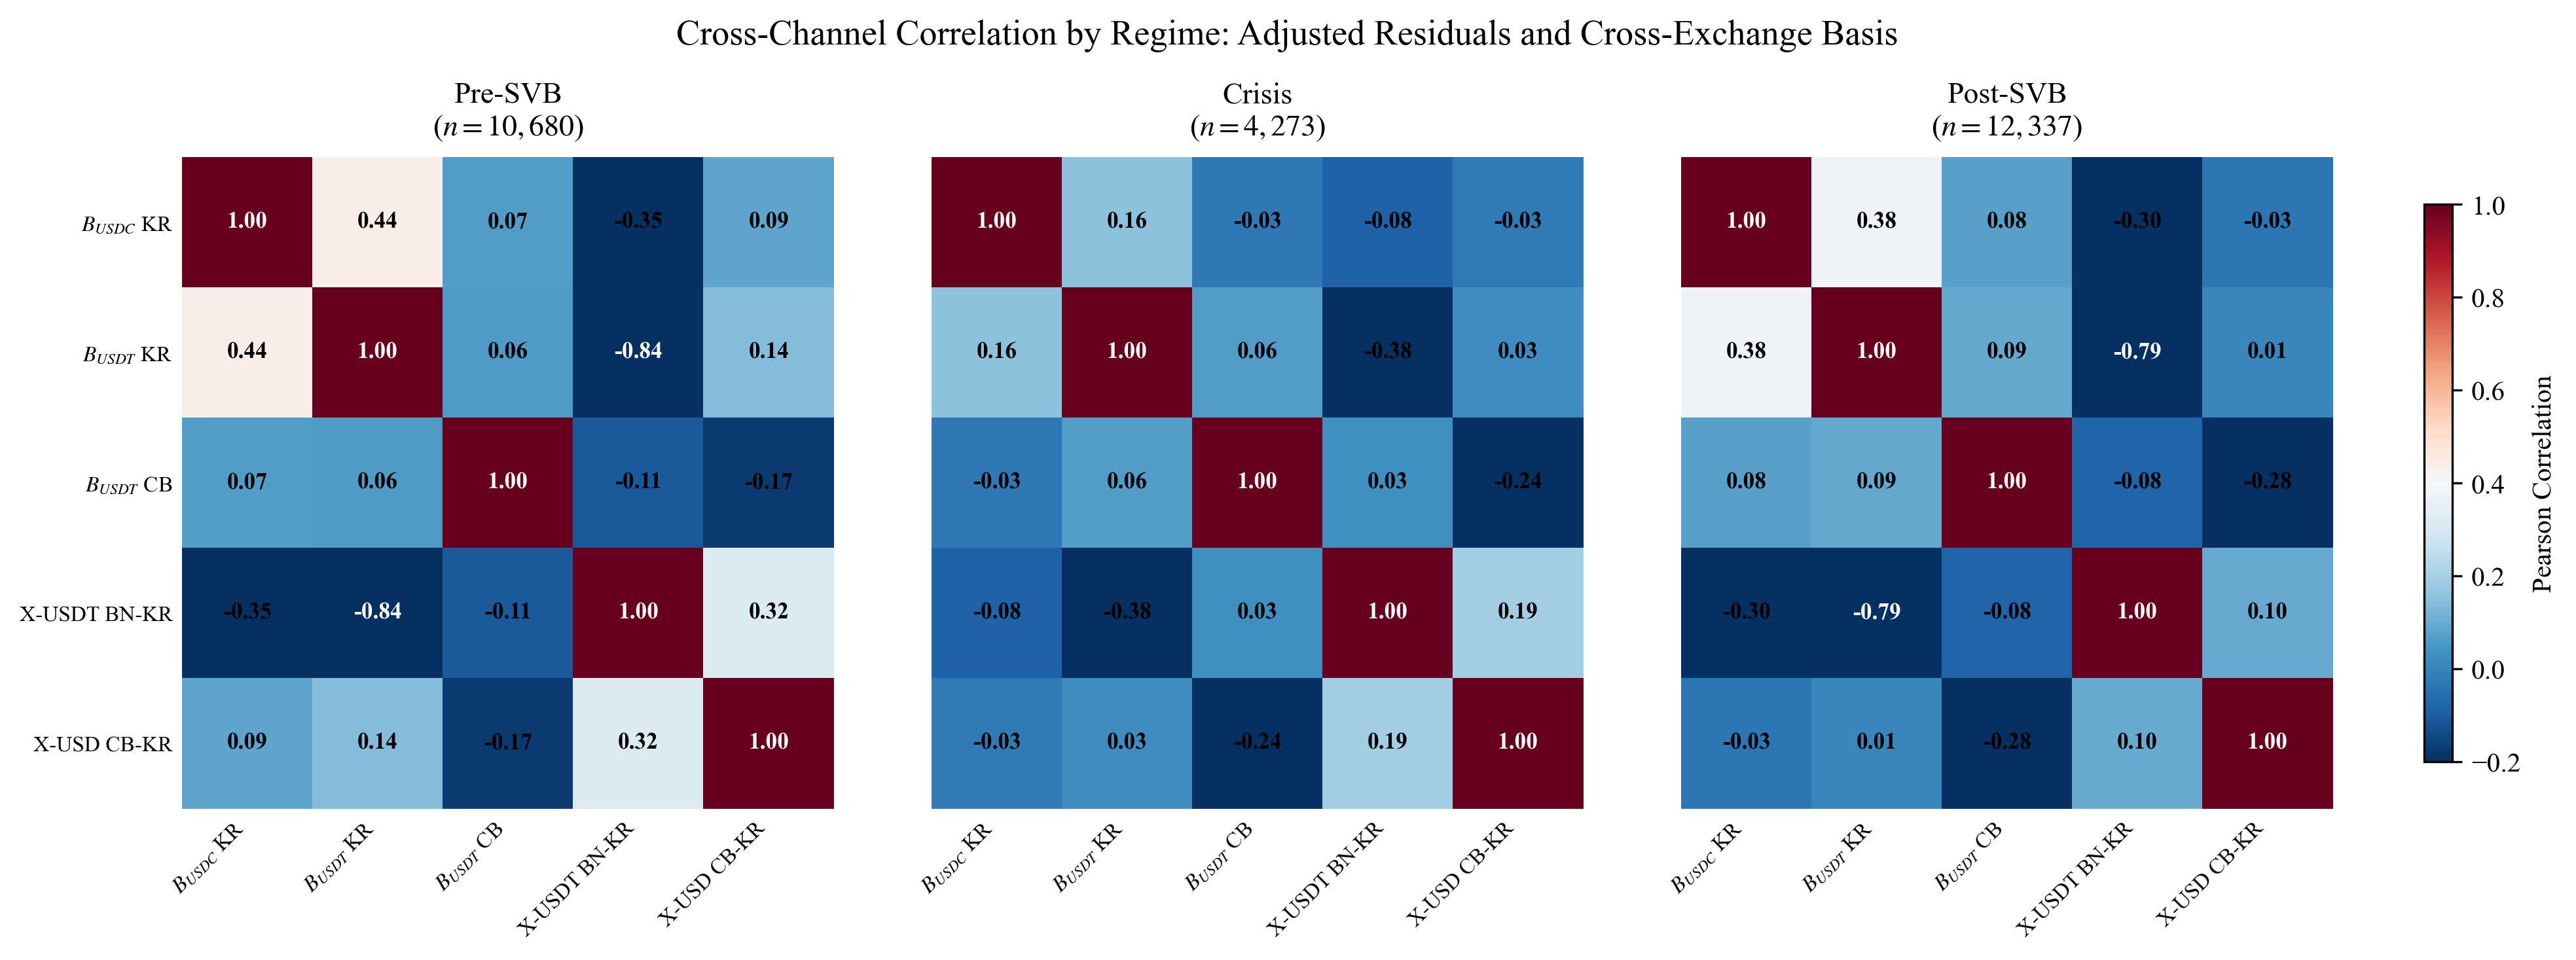
\includegraphics[width=0.95\linewidth]{figures/fig_correlation_regime_heatmap.png}
    \caption{Cross-channel correlation by regime for adjusted residuals and cross-exchange basis. The $B_{\text{USDC}}$--$B_{\text{USDT}}$ correlation collapses from $0.44$ (pre-SVB) to $0.16$ (crisis), consistent with divergent stablecoin dynamics rather than a common shock.}
    \label{fig:corrheat}
\end{figure}

\subsection{Price discovery}
Given the liquidity asymmetry documented above---Coinbase BTC/USD is $26\times$ deeper than Kraken BTC/USDC---a natural question is where price discovery occurs across these fragmented channels.

\begin{table}[H]
\caption{Johansen Cointegration and VECM Price Discovery (Primary Kraken Channels, No-FF Sample)}
\label{tab:coint_vecm}
\footnotesize
\centering
\begin{tabular}{lccccccl}
\toprule
Channel & Rank & $k_\Delta$ & Trace$_{r=0}$ & $\alpha_{\text{USD}}$ & $\alpha_{\text{other}}$ & IS$_{\text{USD}}$ [0.69, 0.77] & Leader \\
\midrule
BTC/USD vs BTC/USDC & 0 & 2 & 7.71 & --- & --- & --- & undetermined \\
BTC/USD vs BTC/USDT & 1 & 8 & 27.03 & 0.0079 & 0.0118 & 0.73 & BTC/USD \\
\bottomrule
\multicolumn{8}{l}{\footnotesize 95\% critical value for trace $r=0$: 15.49. IS = Hasbrouck (1995) midpoint; bounds [0.69, 0.77].}
\end{tabular}
\end{table}


Table~\ref{tab:coint_vecm} shows Kraken BTC/USD vs.\ BTC/USDT rejects no cointegration (rank $=1$; stable at $k_\Delta\pm1$). Hasbrouck (1995) IS bounds via both Cholesky orderings \cite{hasbrouck1995}: IS$_{\text{USD}}\in[0.69,\,0.77]$, midpoint $\mathbf{0.73}$---BTC/USD accounts for ${\approx}73\%$ of permanent price discovery. Bounds are tight (width $0.08$), so leadership is not ordering-driven. Residual correlation $0.889$ confirms high co-movement. For BTC/USD vs.\ BTC/USDC, no-FF does not reject rank $=0$, consistent with long-run instability over this short window.

Figure~\ref{fig:irf} provides complementary visual evidence via orthogonalized impulse-response functions from a bivariate VAR on 1-minute returns (AIC-selected 10 lags; Cholesky ordering: BTC/USD first, consistent with its IS leadership; $N{=}26{,}548$ full-sample observations). A one-standard-deviation shock to BTC/USD transmits significantly to BTC/USDC (Panel~C: ${\approx}6$ bps at impact, decaying within 3--4 minutes), while the reverse channel (Panel~B) is statistically indistinguishable from zero---the 95\% confidence band envelops the zero line at all horizons. This asymmetry is consistent with the Hasbrouck IS finding and confirms that fiat-quoted prices lead stablecoin-quoted prices in the information transmission chain.

\begin{figure}[t]
    \centering
    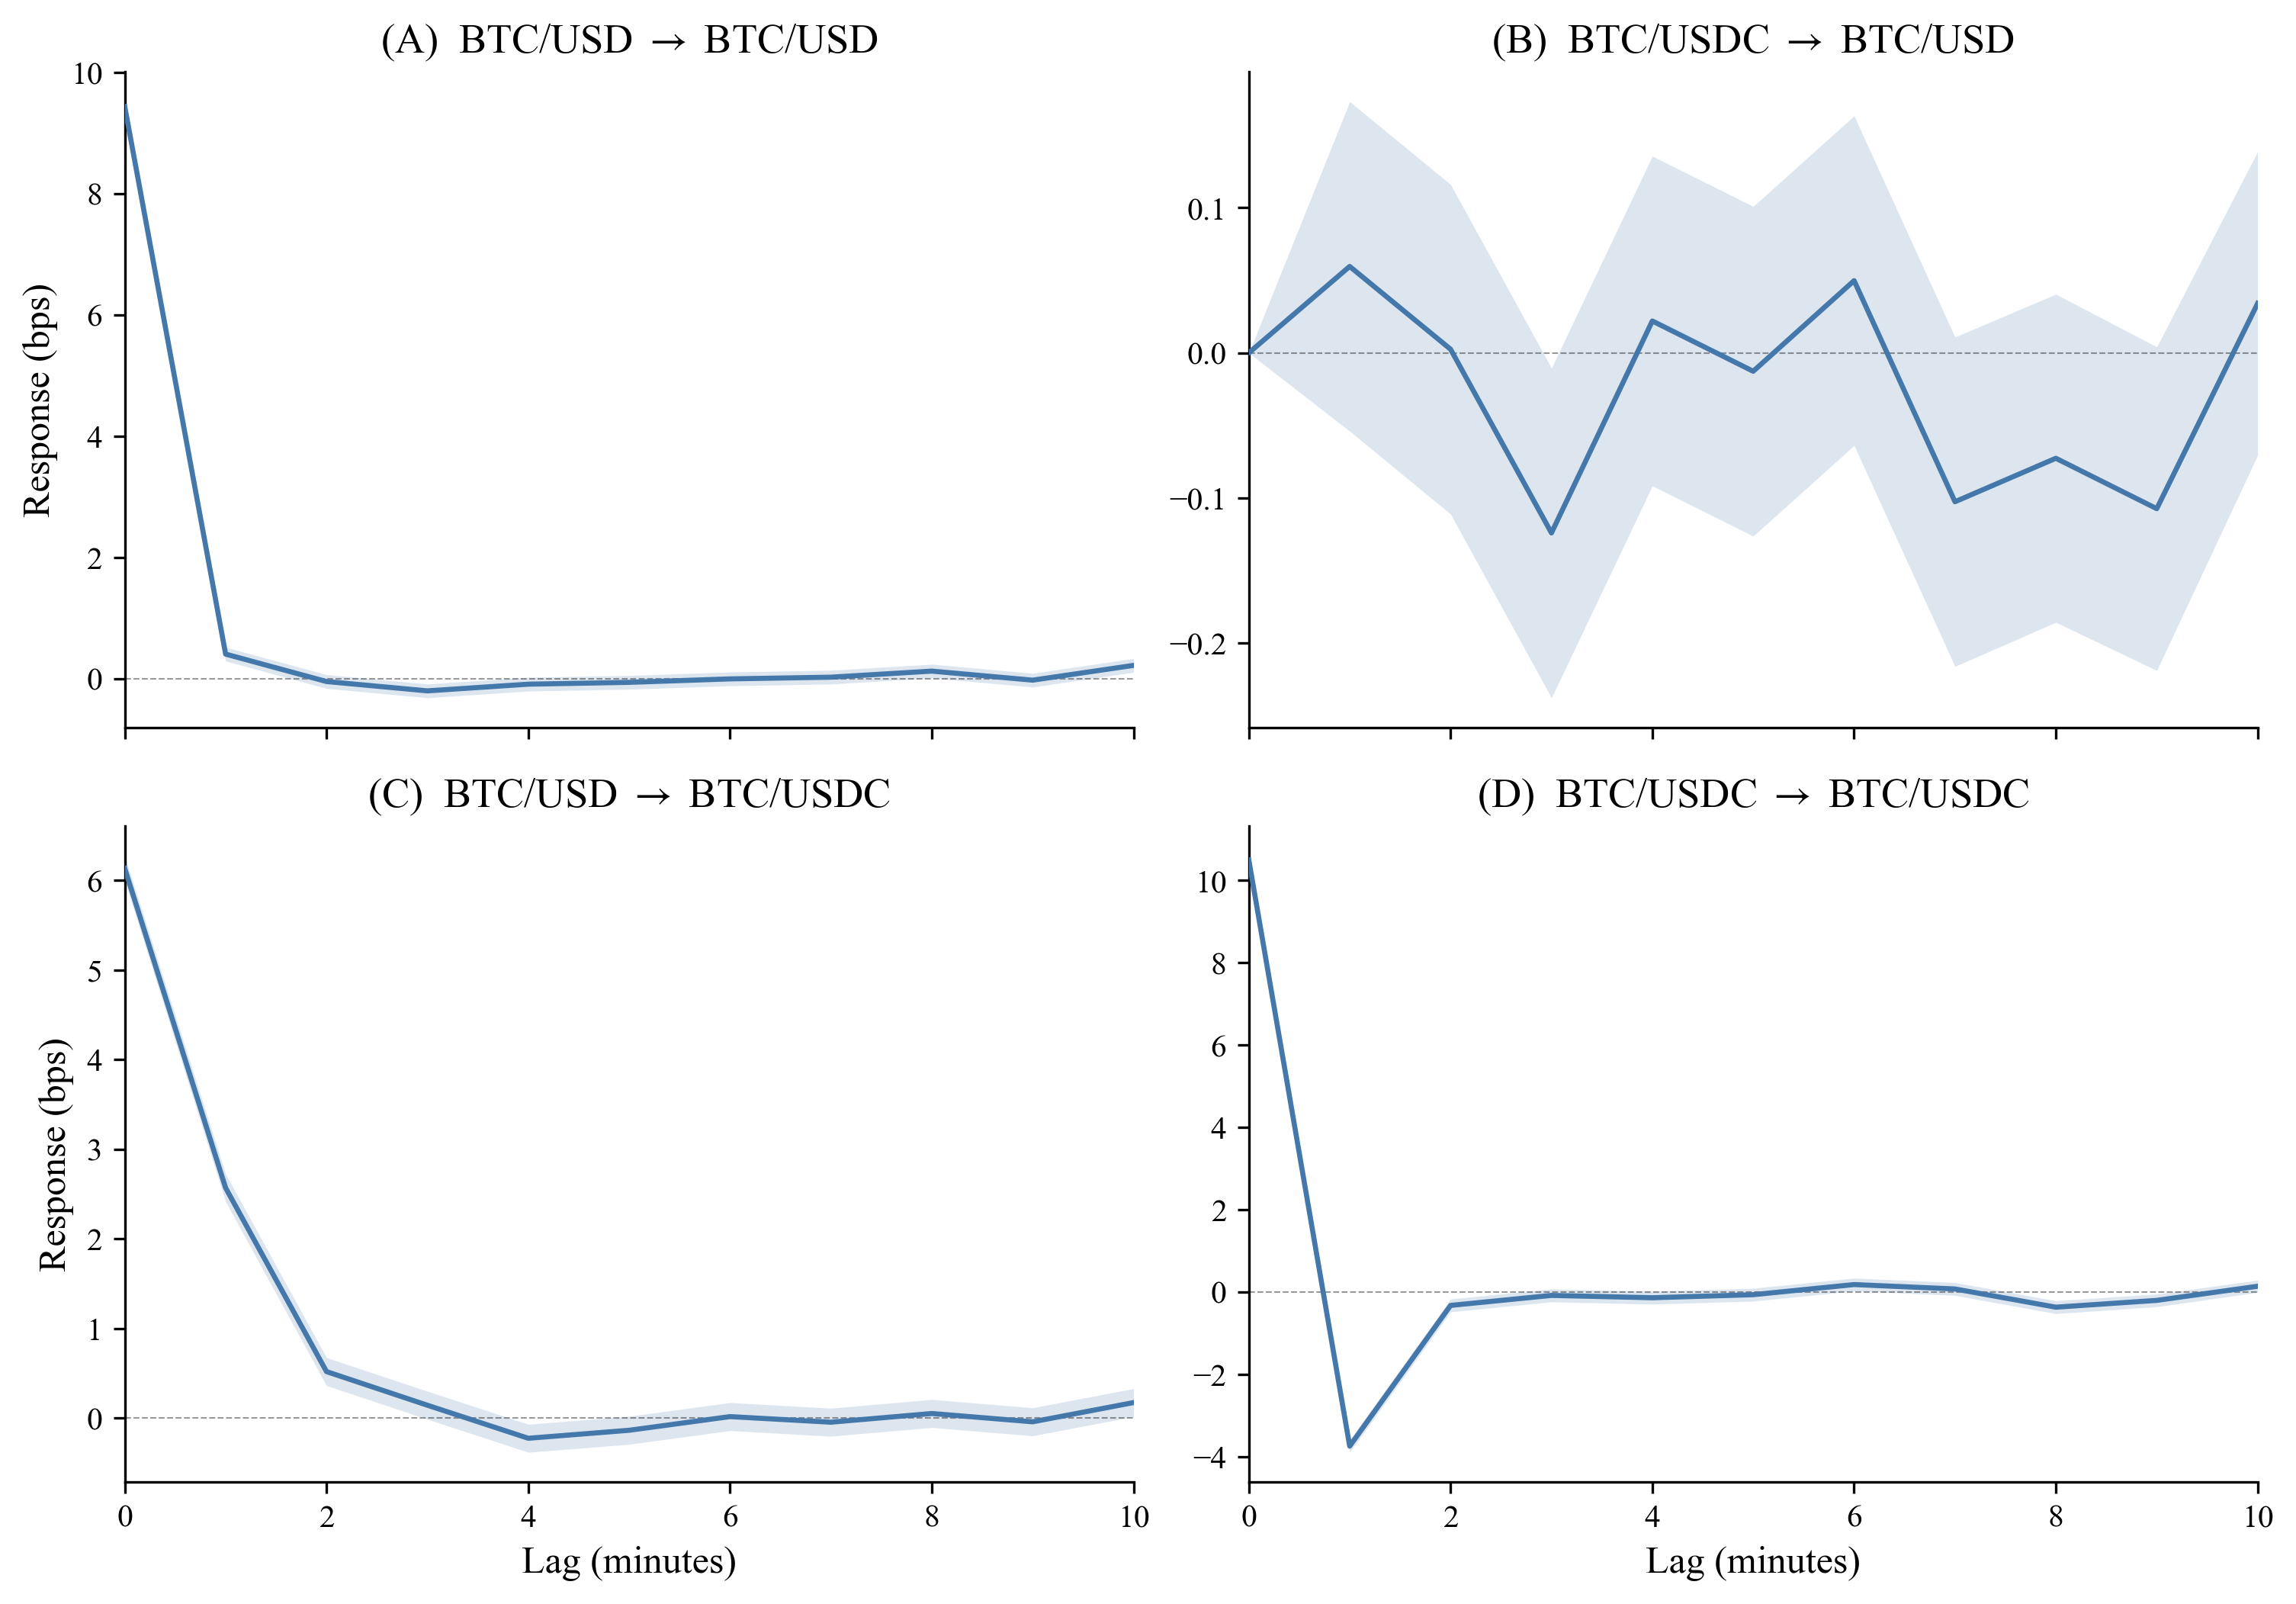
\includegraphics[width=0.92\linewidth]{figures/fig_var_irf.png}
    \caption{Orthogonalized impulse-response functions from bivariate VAR(10) on Kraken BTC/USD and BTC/USDC 1-minute returns (bps). (A)~Own BTC/USD persistence. (B)~BTC/USDC $\to$ BTC/USD: insignificant (CI includes zero). (C)~BTC/USD $\to$ BTC/USDC: significant transmission (${\approx}6$ bps, decays in 3--4 min). (D)~Own BTC/USDC response with partial reversal at lag 1. Shaded: 95\% asymptotic CI.}
    \label{fig:irf}
\end{figure}

BH/FDR-corrected Granger tests on returns provide secondary evidence: BTC/USD $\to$ BTC/USDC is significant ($q<0.001$) but the reverse is not after FDR correction ($q=0.13$), consistent with fiat-to-stablecoin price adjustment. All other channels (USDT intra-exchange, cross-exchange) show bidirectional significance, consistent with active two-way arbitrage in more liquid markets.

\subsection{Arbitrage after fees}\label{sec:arb}
Having established that price discovery resides in the fiat-quoted channel, a natural question is whether the documented dislocations offer exploitable arbitrage opportunities. We evaluate this using explicit trade construction---3-leg triangular for intra-exchange stablecoin channels, 2-leg pre-funded buy/sell for cross-exchange---under two cost bounds:
\begin{align}
    \text{cost}^{\text{fee}}_t &= n_{\text{legs}}\cdot f, \\
    \text{cost}^{\text{fee+slip}}_t &= n_{\text{legs}}\cdot f + \sum_{\ell=1}^{n_{\text{legs}}}\tfrac{1}{2}\,\text{RangeProxy}_{\ell,t},
\end{align}
with $f=5$ bps per taker leg.

\begin{table}[H]
\caption{Arbitrage Profitability by Channel and Regime (5 bps/leg; 3-leg intra-exchange, 2-leg cross-exchange)}
\label{tab:arb}
\begin{tabular}{llcrr}
\toprule
Channel & Regime & Cost Variant & \%Profitable & AvgNetUncond (bps) \\
\midrule
USDC/USD (Kraken) & Crisis & Fee-only & 29.16 & 4.83 \\
USDC/USD (Kraken) & Crisis & Fee+slip & 6.72 & 0.64 \\
USDC/USD (Kraken) & Post-SVB & Fee-only & 9.38 & 0.56 \\
USDC/USD (Kraken) & Post-SVB & Fee+slip & 1.78 & 0.08 \\
USDT/USD (Kraken) & Crisis & Fee-only & 3.76 & 0.14 \\
USDT/USD (Kraken) & Crisis & Fee+slip & 0.37 & 0.01 \\
Cross BTC/USD (CB--KR) & Crisis & Fee-only & 11.32 & 0.72 \\
Cross BTC/USD (CB--KR) & Crisis & Fee+slip & 2.29 & 0.15 \\
Cross BTC/USDT (BN--KR) & Crisis & Fee-only & 11.85 & 0.49 \\
Cross BTC/USDT (BN--KR) & Crisis & Fee+slip & 1.81 & 0.05 \\
\bottomrule
\end{tabular}
\end{table}


Figure~\ref{fig:arbfees} shows the time series of net arbitrage profits under both cost specifications. Adding range-based slippage (Panel~B) materially compresses profitability: USDC intra-exchange crisis profitability falls from $29.16\%$ to $6.72\%$ (net $4.83$ to $0.64$ bps); Coinbase--Kraken BTC/USD falls from $11.32\%$ to $2.29\%$. Fee sensitivity: at $f{=}3$ bps (maker rebate), USDC crisis fee+slippage profitability rises to $14.0\%$; at $f{=}10$ bps (retail), it falls to $1.0\%$. The narrow post-cost opportunities are consistent with limited executable arbitrage under realistic frictions.

\begin{figure}[t]
    \centering
    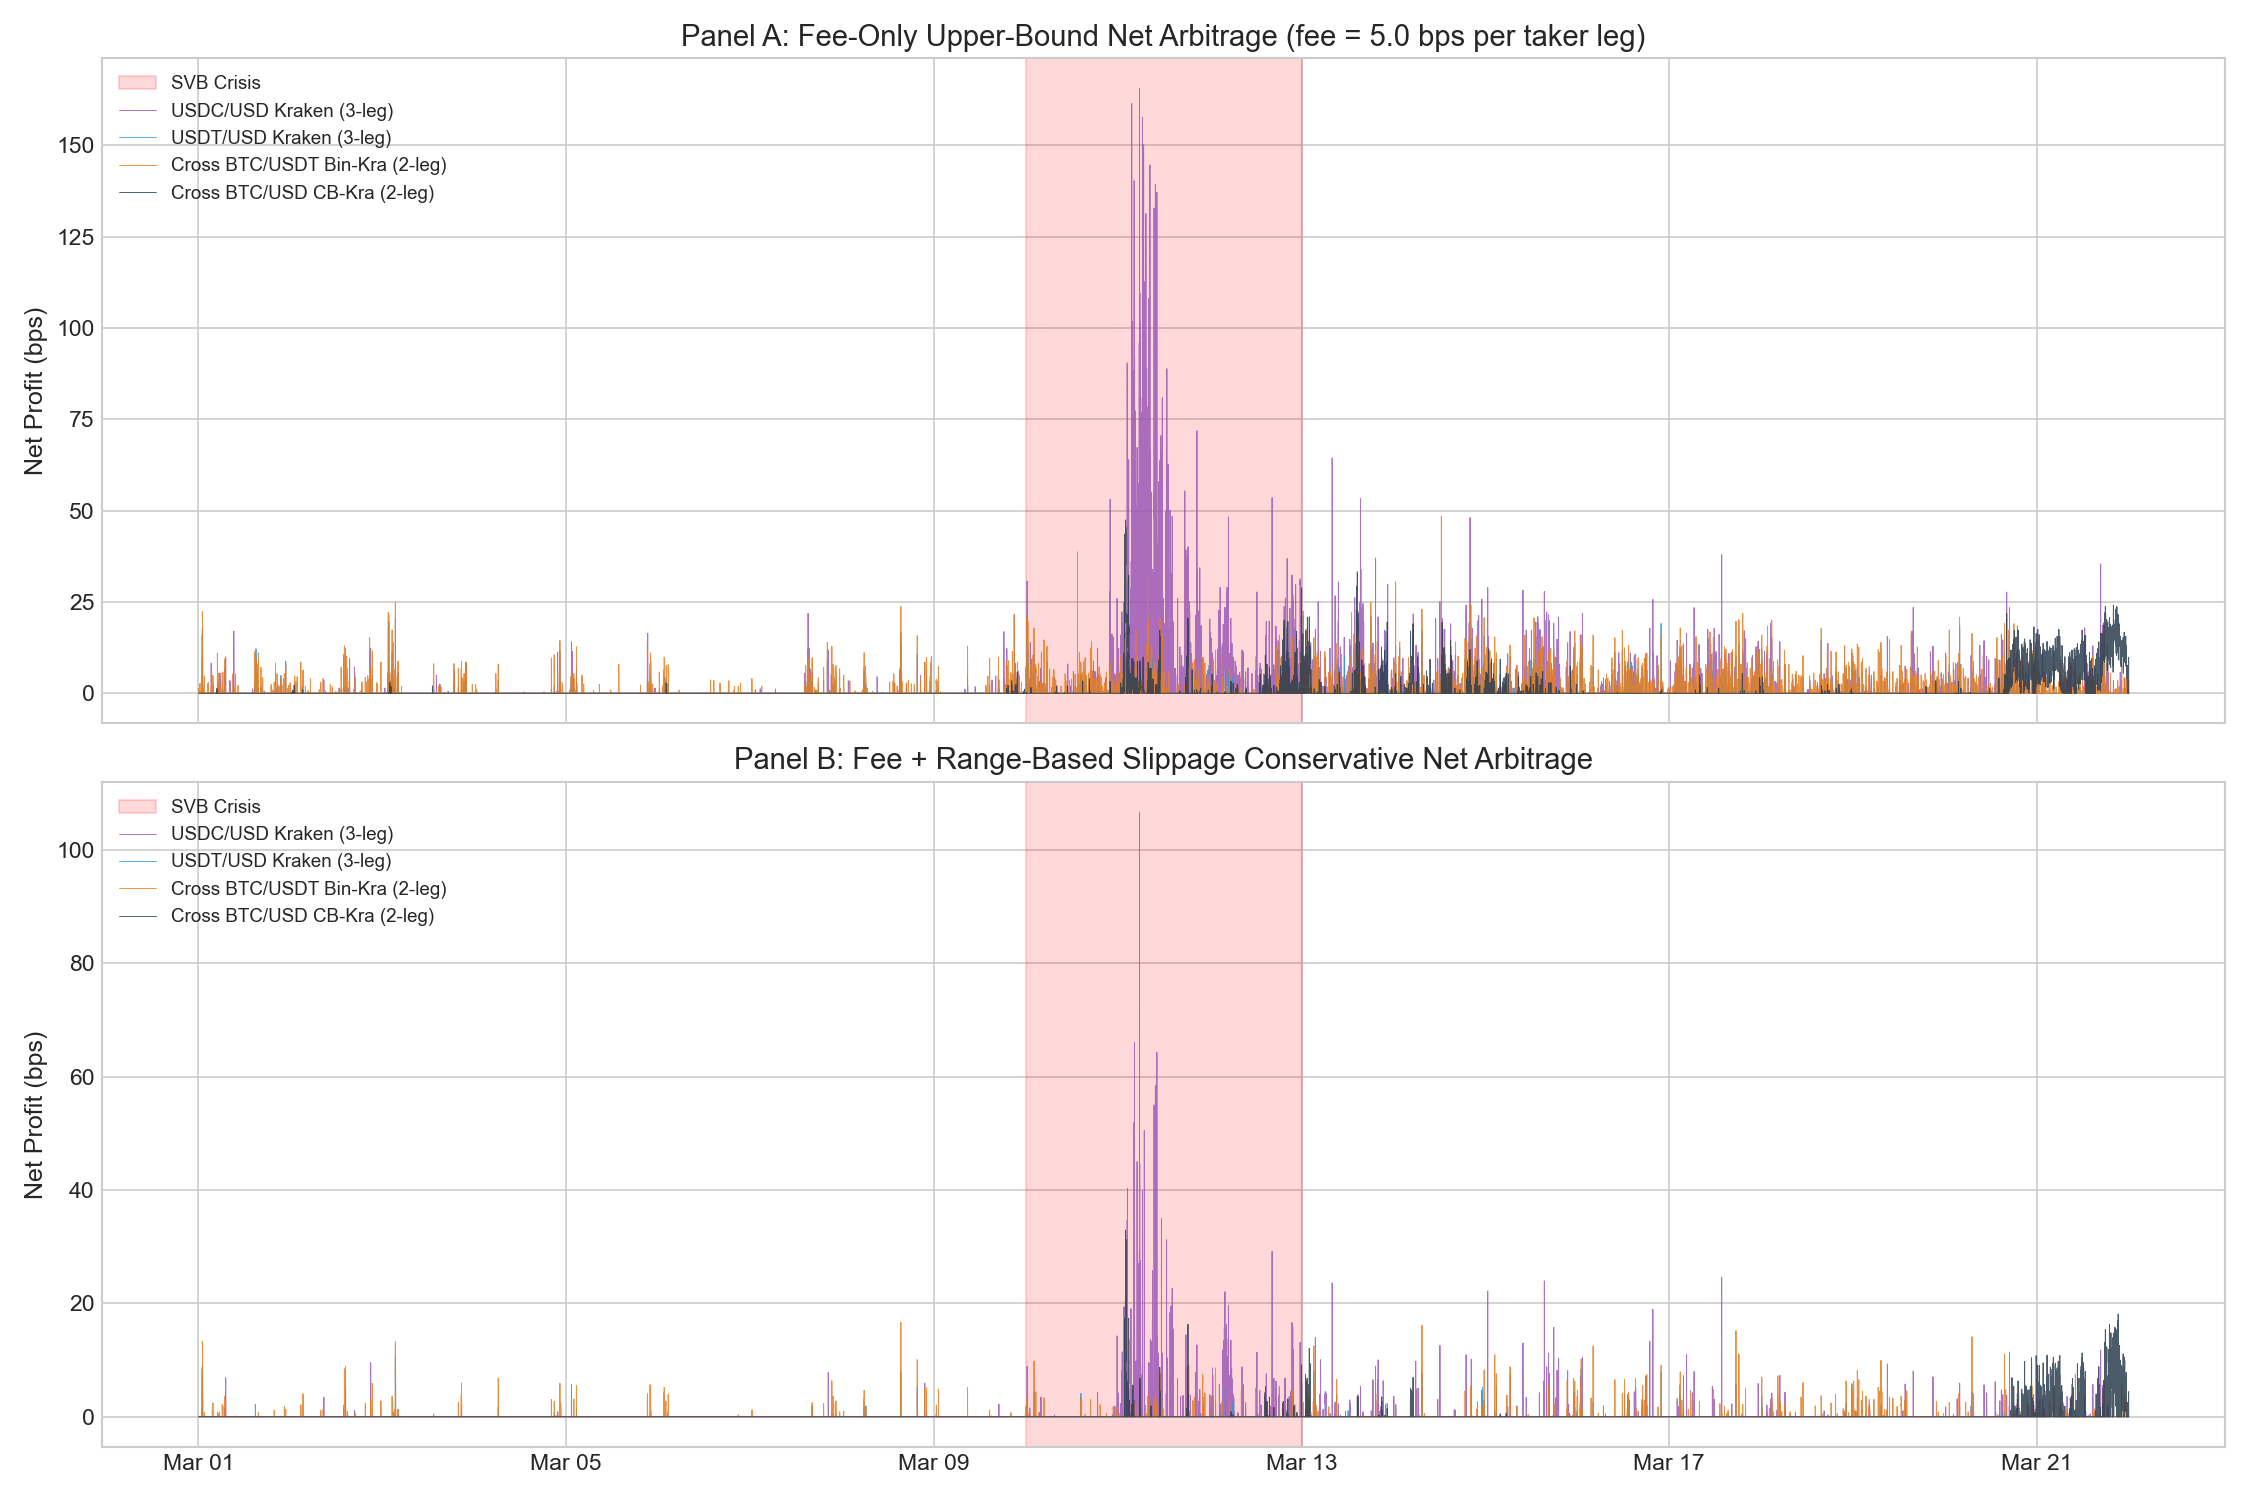
\includegraphics[width=0.92\linewidth]{figures/fig_arbitrage_after_fees.png}
    \caption{Arbitrage net profit (bps) over time. Panel~A: fee-only (5 bps/leg); Panel~B: fee + range-based slippage. The USDC intra-exchange channel (orange) spikes during crisis but collapses under slippage. Cross-exchange profits (dashed) are similarly attenuated.}
    \label{fig:arbfees}
\end{figure}

\section{Regulatory Interpretation}\label{sec:regulation}

The preceding analysis identifies a clear failure chain: reserve-access risk drives peg deviation, peg deviation drives dispersion, and limited depth constrains arbitrage correction. We now ask whether the GENIUS Act's provisions target this chain. The results point to banking-layer reserve-access risk as the root cause. Circle held \$3.3B (${\approx}8\%$) of USDC reserves at SVB \cite{circle2023}; the ${\sim}940\times$ half-life gap localizes persistent dislocation to the peg layer. Sustained recovery required emergency deposit guarantees on March 16 \cite{jointstatement2023}.

The GENIUS Act (July 2025) targets four dimensions of this chain; we map provisions to results as consistency checks \cite{genius2025}. (i)~\emph{Reserve composition}: Table~\ref{tab:genius_cf} maps 25\%--75\% mitigation to implied $D_t$ of ${\approx}240$--$80$ bps. (ii)~\emph{Timely redemption}: the $572$-min peg half-life (vs.\ $1.06$ pre-SVB) quantifies the five-day redemption freeze. (iii)~\emph{Bankruptcy super-priority}: targets P99 tail risk ($81.4$ vs.\ $13.6$ bps). (iv)~\emph{Transparency}: traders learned of SVB exposure only from Circle's Friday-night disclosure, consistent with the USDC--USDT decorrelation ($\rho{=}0.16$).

\begin{table}[H]
\caption{GENIUS Act scenario range (illustrative, not structural causal identification). The table maps assumed mitigation of reserve lock-up shock into implied crisis $D_t$ means, anchored to observed pre- and crisis-period moments. Tail benchmark for context: USDC $B_t$ crisis P99 = 81.4 bps versus pre-crisis P99 = 13.6 bps.}
\label{tab:genius_cf}
\footnotesize
\resizebox{\textwidth}{!}{%
\begin{tabular}{p{3.3cm}rrrp{4.5cm}}
\toprule
Scenario & Assumed mitigation of lock-up shock (\%) & Implied crisis D\_t mean (bps) & Reduction vs observed (bps) & Policy mapping \\
\midrule
Observed baseline & 0 & 320.0 & 0.0 & SVB/No GENIUS baseline \\
Low mitigation & 25 & 240.0 & 80.0 & Reserve composition + redemption + transparency \\
Moderate mitigation & 50 & 160.0 & 159.9 & Reserve composition + redemption + transparency \\
High mitigation & 75 & 80.1 & 239.9 & Reserve composition + redemption + transparency \\
Full-mitigation lower bound & 100 & 0.1 & 319.9 & Reserve composition + redemption + transparency \\
\bottomrule
\end{tabular}%
}
\end{table}


Persistent cross-exchange deviations ($+2.18$ bps) and the $26\times$ depth gap suggest reserve-layer reforms alone may not eliminate spatial fragmentation.

\section{Conclusion}\label{sec:conclusion}

Three findings emerge. First, SVB-triggered fragmentation is attributable to stablecoin peg risk: $D_t$ reaches $+320$ bps but $B_t$ stays near $+5$ bps with sub-minute mean reversion; the ${\sim}940\times$ half-life gap localizes persistent dislocation to reserve-access risk. Second, the crisis is USDC-specific: excess kurtosis $12.9$ ($6\times$ tail expansion), USDT safe-haven premium ($+58$ bps), and cross-stablecoin decorrelation ($0.44\to0.16$). Third, post-friction arbitrage narrows sharply ($29\%\to7\%$), with the $26\times$ depth gap limiting executable scale.

The GENIUS Act's provisions target precisely this failure chain. Because dislocation resides in the peg layer, reforms reducing reserve-access risk should compress $D_t$ more effectively than measures targeting cross-market efficiency. However, persistent cross-exchange deviations and depth asymmetry suggest additional market-structure measures may also be needed. A natural next step is a post-GENIUS replication study during the next stress event.

\paragraph{Interpretation boundaries.} This evidence is window-specific (March~2023) and observational; policy passages are consistency mappings, not causal identification.
Robustness: (i)~HAC intervals preserve directional signs; (ii)~no-FF filters preserve rank-order conclusions; (iii)~cointegration is rank-stable for BTC/USD--USDT but not USDC; (iv)~Chow tests confirm the regime split.

\smallskip\noindent\textbf{Reproducibility.}
All exhibits are deterministic outputs of \texttt{run\_all.py}; artifact-label integrity is verified by \texttt{src/04\_tex\_integrity\_check.py}.

\small
\begin{thebibliography}{99}
\bibitem{amihud2002} Amihud, Y. (2002). Illiquidity and stock returns: Cross-section and time-series effects. \emph{Journal of Financial Markets}, 5(1), 31--56.
\bibitem{chow1960} Chow, G. C. (1960). Tests of equality between sets of coefficients in two linear regressions. \emph{Econometrica}, 28(3), 591--605.
\bibitem{circle2023} Circle (March 11, 2023). \emph{Silicon Valley Bank and USDC}. Circle update.
\bibitem{englegranger1987} Engle, R. F., \& Granger, C. W. J. (1987). Co-integration and error correction: Representation, estimation, and testing. \emph{Econometrica}, 55(2), 251--276.
\bibitem{jointstatement2023} Federal Reserve, FDIC, and U.S. Treasury (March 12, 2023). \emph{Joint statement by the Department of the Treasury, Federal Reserve, and FDIC}.
\bibitem{granger1969} Granger, C. W. J. (1969). Investigating causal relations by econometric models and cross-spectral methods. \emph{Econometrica}, 37(3), 424--438.
\bibitem{hasbrouck1995} Hasbrouck, J. (1995). One security, many markets: Determining the contributions to price discovery. \emph{Journal of Finance}, 50(4), 1175--1199.
\bibitem{johansen1988} Johansen, S. (1988). Statistical analysis of cointegration vectors. \emph{Journal of Economic Dynamics and Control}, 12(2--3), 231--254.
\bibitem{neweywest1987} Newey, W. K., \& West, K. D. (1987). A simple, positive semi-definite, heteroskedasticity and autocorrelation consistent covariance matrix. \emph{Econometrica}, 55(3), 703--708.
\bibitem{roll1984} Roll, R. (1984). A simple implicit measure of the effective bid-ask spread in an efficient market. \emph{Journal of Finance}, 39(4), 1127--1139.
\bibitem{genius2025} U.S. Congress (2025). \emph{Public Law 119-27: Guiding and Establishing National Innovation for U.S. Stablecoins Act (GENIUS Act)}.
\end{thebibliography}

\end{document}
